\chapter{Resultados}
\label{cap:resultados}

Este capítulo apresenta os resultados da análise das séries temporais de 
precipitação acumulada, temperatura média e radiação solar incidente em 
superfície nos estados de São Paulo e Rio Grande do Norte para o período 
1990-2024.

Primeiramente, apresenta-se a avaliação da correlação entre dados observacionais 
de estações meteorológicas (INMET e ANA) e dados de satélite e reanálise 
(CHIRPS, CLARA-A3 e ERA5-Land) para o período 2004-2024. Este intervalo foi selecionado por corresponder ao período de maior consistência 
e densidade das observações do INMET. Para esta análise, utilizou-se o 
método de Regressão de Distância Ortogonal, seguindo os passos empregados no Capítulo \ref{cap:metodologia}.

Em seguida, foi feito o processo de caracterização espacial das tendências climáticas 
através de análises estatísticas aplicadas aos dados de satélite e reanálise.
Para obtenção das tendências temporais, aplicou-se o teste 
de Mann-Kendall, e para quantificação da magnitude destas tendências, 
utilizou-se o estimador de Sen.

Na terceira parte é apresentada a caracterização das normais climatológicas calculadas 
para o período completo de análise (1990-2024), que contextualizam os valores 
médios e a variabilidade de cada variável climática. 

Após compreender as implicações dos resultados anteriores e que a partir daqui sucedem, foram aplicados métodos de identificação da magnitude relativa das tendências observadas juntamente com as transformações documentadas no uso e 
cobertura da terra ao longo do período analisado.

Adicionalmente, foram investigadas as respostas das variáveis climáticas em áreas caracterizadas por extremos de mudança no uso e cobertura da terra, com base nos percentis superiores e inferiores de variação das classes dominantes em cada estado.

Para o estado de São Paulo, a análise concentrou-se principalmente na classe de Formação Florestal, enquanto no Rio Grande do Norte o foco voltou-se sobre a Formação Savânica (Caatinga), refletindo as características predominantes de cada bioma. A evolução temporal das variáveis climáticas nessas áreas foi avaliada de forma integrada, permitindo identificar diferenças sistemáticas associadas às transformações da superfície.

Em uma etapa subsequente, realizou-se uma avaliação quantitativa da relação entre as mudanças na cobertura da superfície e as variáveis climáticas, por meio de ajustes estatísticos aplicados às séries temporais agregadas em pontos de grade. Essa análise teve como objetivo estimar a magnitude relativa da influência das diferentes classes de uso da terra sobre as tendências observadas de temperatura, precipitação e radiação solar, considerando a variabilidade espacial e temporal dos dados.

Por fim, os resultados foram sintetizados de forma comparativa entre os estados de São Paulo e Rio Grande do Norte, destacando semelhanças e contrastes nos padrões de resposta climática associados às mudanças de uso e cobertura da terra.


\section{Análise de correlão entre os dados observacionais e produtos de Satélite e Reanálise}

Antecedento ao procedimento de análise de tendências climáticas, considerou-se um processo de validação cruzada entre dados observacionais de estações meteorológicas (INMET e ANA) e produtos derivados de satélite e reanálise (CHIRPS, CLARA-A3, GOES-16 e ERA5-Land) para o período comum de sobreposição 2004-2024. Esta validação foi utilizada com o objetivo de cobrir as seguintes questões: primeiro, para confirmar que os produtos de sensoriamento remoto reproduzem adequadamente a variabilidade climática observada localmente pelas estações físicas; segundo, para quantificar as incertezas associadas aos diferentes produtos que serão posteriormente utilizados nas análises de tendências espaciais; e terceiro, para identificar eventuais vieses sistemáticos que possam requerer correção ou que devam ser considerados na interpretação dos resultados. Além disso, vale salientar a importância da agregação de diversas fontes justamente pela limitação encontrada em diversos pontos do Brasil, principalmente pela falta de manutenção e acompanhamento de equipamentos de monitoramento em terra.

A metodologia de validação empregou regressão ortogonal por distância (Orthogonal Distance Regression, ODR) \cite{boggs1990odr}, técnica essa que como mencionada em Metodologias visa descrever a primeiramente mesmo que de forma indireta a diferença quando comparada a regressão linear ordinária por considerar explicitamente as incertezas em ambas as variáveis (observações e estimativas satelitais), ao invés de assumir que apenas a variável dependente possui erro significativo. Como já destacado em outros pontos deste estudo, esta abordagem é particularmente apropriada no presente contexto, onde tanto as medições de estações quanto as estimativas de satélite estão sujeitas a incertezas não desprezíveis e por também ser um método pouco usado em estudos na área de meteorologia, que em geral utiliza-se o ajuste linear para a validação de diferentes fontes.

Os ajustes foram avaliados com base em múltiplos indicadores estatísticos complementares: o coeficiente de correlação de Pearson ($R$) que quantifica a intensidade da associação linear entre as variáveis; o qui-quadrado reduzido ($\chi^2_r$) que avalia a qualidade do ajuste considerando as incertezas estimadas, com valores próximos a 1 indicando consistência estatística adequada entre modelo e dados \citep{press2007numerical}; e o número de pares de dados ($N$) que estabelece a significância estatística dos resultados. Os parâmetros de regressão (coeficiente angular e linear) foram reportados com suas incertezas estimadas pelo método ODR.

\subsection{Correlação entre precipitação observada (ANA) e estimada por satélite (CHIRPS)}

A validação da precipitação baseou-se na comparação entre dados pluviométricos acumulados anuais provenientes de estações convencionais da Agência Nacional de Águas (ANA) e estimativas do produto CHIRPS (Climate Hazards Group InfraRed Precipitation with Station data), combinando os dados de observações de satélite infravermelho com dados de estações para produzir campos espacialmente contínuos de precipitação \citep{funk2015}.

\begin{figure}[htbp]
	\centering
	\begin{minipage}{0.6\textwidth}
		\centering
		\includegraphics[width=\textwidth]{cor_ana_sp.png}
		
		(a) São Paulo
	\end{minipage}
	\hfill
	\begin{minipage}{0.6\textwidth}
		\centering
		\includegraphics[width=\textwidth]{cor_ana_rn.png}
		
		(b) Rio Grande do Norte
	\end{minipage}
	\caption{Correlação entre precipitação acumulada anual observada em estações da ANA e estimada pelo produto CHIRPS para o período 2004–2024.}
	\label{fig:corr_prec_chirps}
\end{figure}

Para o estado de São Paulo (Figura~\ref{fig:corr_prec_chirps}a), a regressão ortogonal entre ANA e CHIRPS resultou em $y = (0{,}544 \pm 0{,}006)x + (581,0 \pm 7,8)$ mm, com coeficiente de correlação moderado $R = 0{,}7$ e qui-quadrado reduzido $\chi^2_r = 0{,}8$, baseado em um conjunto de $N = 3777$ pares de dados. O coeficiente angular substancialmente inferior à unidade ($0{,}544 \pm 0{,}006$) indica tendência sistemática pronunciada do CHIRPS em subestimar os acumulados de precipitação mais elevados, comportamento frequentemente observado em produtos de satélite quando confrontados com eventos convectivos intensos que podem saturar os sensores infravermelhos ou exceder os limites de detecção dos algoritmos de estimativa. O coeficiente linear excepcionalmente elevado de $(581,0 \pm 7,8)$ mm sugere compensação desta subestimação através de viés aditivo substancial que afeta uniformemente toda a faixa de precipitações, resultando em superestimativa de eventos de baixa intensidade.

A dispersão observada nos dados, embora resulte em correlação moderada, pode ser esperada considerando-se: (i) a diferença fundamental nas escalas de representatividade espacial entre medições pontuais de pluviômetros (tipicamente círculos de 20 cm de diâmetro) e pixels CHIRPS de aproximadamente 5 km de resolução espacial, diferença que se torna particularmente problemática para precipitações convectivas de pequena escala espacial; (ii) a heterogeneidade topográfica significativa do estado de São Paulo, incluindo Serra do Mar e Serra da Mantiqueira, que induz gradientes pluviométricos pronunciados em escalas menores que a resolução CHIRPS; e (iii) a variabilidade temporal sub-diária da precipitação convectiva que pode resultar em diferenças substanciais entre acumulações diárias mesmo quando os totais mensais ou anuais são similares.


Já para o Rio Grande do Norte (Figura~\ref{fig:corr_prec_chirps}b), a validação revelou comportamento substancialmente distinto, com regressão ortogonal $y = (0{,}73 \pm 0{,}02)x + (147,2 \pm 9,9)$ mm, correlação notavelmente elevada $R = 0{,}9$ quando comparada ao observado para o estado de São Paulo, qui-quadrado reduzido próximo ao ideal $\chi^2_r = 1,1$, baseado em $N = 229$ pares de dados, consideravelmente inferior aos pares de SP. A correlação superior observada no Rio Grande do Norte comparada a São Paulo aparenta, à primeira vista, contraditória dado que RN possui densidade de estações meteorológicas substancialmente inferior. No entanto, esta diferença reflete por algumas questões como a natureza distinta dos regimes de precipitação dominantes: enquanto São Paulo caracteriza-se por precipitação convectiva intensa e localizada com alta variabilidade espacial, o Rio Grande do Norte apresenta precipitações frequentemente associadas a sistemas de escala sinótica (Zona de Convergência Intertropical, perturbações de leste) que produzem comportamentos mais coerentes, ou seja, separados por apenas "duas estações" características, verão quente e chuvoso e inverno frio e seco, onde portanto, mais adequadamente capturados por produtos de resolução moderada como CHIRPS \citep{kousky1980diurnal}.

O coeficiente angular de $0{,}73 \pm 0{,}02$ no Rio Grande do Norte, embora ainda inferior à unidade, mostra menor subestimação que São Paulo, indicando melhor desempenho do CHIRPS em capturar a magnitude dos eventos de precipitação no semiárido. O coeficiente linear moderado de $(147,2 \pm 9,9)$ mm é substancialmente inferior ao observado em São Paulo, sugerindo menor tendência de super estimativa de precipitações leves. Esta diferença pode estar relacionada tanto às características distintas dos regimes pluviométricos quanto aos processos de calibração do CHIRPS, que utiliza dados de estações pluviométricas locais para ajuste das estimativas de satélite e pode ter maior densidade de estações de calibração disponíveis em regiões semiáridas globalmente similares ao nordeste brasileiro \citep{funk2015}.

\subsection{Correlação entre temperatura média observada (INMET) e reanálise (ERA5-Land)}

A validação da temperatura do ar baseou-se na comparação entre médias diárias observadas em estações automáticas do INMET e dados de reanálise ERA5-Land, produto com resolução espacial sendo de aproximadamente 9 km que assimila observações meteorológicas globais em modelo numérico para produzir campos espaciotemporalmente consistentes de variáveis atmosféricas e de superfície \citep{munoz2021era5}.

\begin{figure}[htbp]
	\centering
	\begin{minipage}{0.6\textwidth}
		\centering
		\includegraphics[width=\textwidth]{correlacao_inmet_era5_tavg_2004_2024_sp.png}
		
		(a) São Paulo
	\end{minipage}
	\hfill
	\begin{minipage}{0.6\textwidth}
		\centering
		\includegraphics[width=\textwidth]{correlacao_inmet_era5_tavg_2004_2024.png}
		
		(b) Rio Grande do Norte
	\end{minipage}
	\caption{Correlação entre temperatura média anual observada em estações automáticas do INMET e dados de reanálise ERA5-Land para o período 2004--2024.}
	\label{fig:corr_temp_era5}
\end{figure}


Para São Paulo (Figura~\ref{fig:corr_temp_era5}a), a regressão ortogonal entre INMET e ERA5-Land para o período 2004-2024 resultou em ajuste acima do adequado $y = (1,0 \pm 0{,}2)x + (0{,}4 \pm 3,4)$ °C, com correlação muito elevada $R = 0{,}9$ e qui-quadrado $\chi^2_r = 4,1$, baseado em $N = 272$ pares de dados anuais representando múltiplas estações distribuídas pelo estado. O coeficiente angular estatisticamente aproximadamente à ($1,0 \pm 0{,}2$) e coeficiente linear próximo a zero ($0{,}4 \pm 3,4$ °C) demonstram baixíssimos vieses sistemáticos significativos, confirmando que ERA5-Land reproduz adequadamente tanto a magnitude quanto a variabilidade da temperatura observada. O qui-quadrado ligeiramente elevado ($\chi^2_r = 4,1$) sugere que as incertezas estimadas podem estar subestimadas ou que existe variabilidade residual não capturada pelo modelo de regressão linear.

No Rio Grande do Norte (Figura~\ref{fig:corr_temp_era5}b), a validação produziu $y = (1,2 \pm 0{,}3)x + (-6,5 \pm 8,5)$ °C, com correlação similar $R = 0{,}9$ mas qui-quadrado mais próximo ao ideal $\chi^2_r = 1,7$, embora baseado em conjunto consideravelmente menor de $N = 56$ pares de dados devido à menor densidade de estações INMET no estado (em contagem). O coeficiente angular ligeiramente superior à unidade ($1,2 \pm 0{,}3$) combinado com intercepto negativo sugere tendência sutil do ERA5-Land em amplificar a amplitude térmica em relação às observações, comportamento que pode estar relacionado às características específicas do modelo de superfície utilizado na reanálise quando aplicado a solos semiáridos com propriedades térmicas distintas daquelas de regiões mais úmidas.

\subsection{Correlação entre radiação solar média observada (INMET) e produtos de satélite (CLARA-A3 e GOES-16)}

A validação da radiação solar incidente na superfície envolveu comparação entre medições piranométricas de estações automáticas do INMET e dois produtos satelitais complementares: CLARA-A3 (CM SAF cLoud, Albedo and surface RAdiation dataset from AVHRR data), derivado de observações de longo prazo do satélite polar AVHRR com resolução espacial de aproximadamente 25 km \citep{karlsson2017clara}, e GOES-16, produto geoestacionário de alta resolução temporal derivado do satélite GOES-16 posicionado sobre a América do Sul. 

A utilização de dois produtos de satélite complementares fundamenta-se em suas características distintas: CLARA-A3, com série temporal desde 1982 e processamento climatológico homogêneo, sendo isso essencial para análises de tendências 
de longo prazo, enquanto GOES-16, operacional desde 2017 com dados  retrospectivos a partir de 2014, representa um intervalo para série temporal inferior quando comparado ao CLARA-A3, mas em termos de resolução espacial o seu perfil é superior, sendo de 500 metros na região do visível, enquanto que para espectros do infravermelho e de vapor d'água a resolução passa a ser de 1 km a 2 km, capturando mais dados atmosféricos em diferentes faixas espectrais.

\begin{figure}[htbp]
	\centering
	\begin{minipage}{0.8\textwidth}
		\centering
		\includegraphics[width=\textwidth]{1.png}
		
		(a) São Paulo
	\end{minipage}
	\par\medskip
	\begin{minipage}{0.8\textwidth}
		\centering
		\includegraphics[width=\textwidth]{4_2.png}
		
		(b) Rio Grande do Norte
	\end{minipage}
	\caption{Correlação entre a radiação solar global medida por estações automáticas do INMET e estimada pelo satélite GOES-16 para o ano de 2014.}
	\label{fig:corr_rad_goes}
\end{figure}

A comparação INMET versus GOES-16 para 2014 (Figura~\ref{fig:corr_rad_goes}) no Rio Grande do Norte (Figura~\ref{fig:corr_rad_goes}b) resultou em $y = (0{,}73 \pm 0{,}02)x + (64 \pm 5)$ W/m$^2$, $R^2 = 0{,}6$, $\chi^2_r = 1,00$ e $N = 1167$, enquanto São Paulo (Figura~\ref{fig:corr_rad_goes}a) apresentou $y = (0{,}79 \pm 0{,}01)x + (27 \pm 1)$ W/m$^2$, $R^2 = 0{,}7$, $\chi^2_r = 1,0$ e $N = 8831$. Os coeficientes angulares sistematicamente inferiores à unidade ($0{,}73$ e $0{,}79$) indicam que GOES-16 tende a subestimar radiação em condições de alta incidência, comportamento potencialmente relacionado à saturação parcial dos sensores ou limitações nos algoritmos de correção atmosférica em atmosferas com aerossóis elevados.

\begin{figure}[htbp]
	\centering
	\begin{minipage}{0.8\textwidth}
		\centering
		\includegraphics[width=\textwidth]{2.png}
		
		(a) São Paulo
	\end{minipage}
	\par\medskip
	\begin{minipage}{0.8\textwidth}
		\centering
		\includegraphics[width=\textwidth]{3.png}
		
		(b) Rio Grande do Norte
	\end{minipage}
	\caption{Correlação entre a radiação solar global medida por estações automáticas do INMET e estimada pelo produto CLARA-A3 para o ano de 2014.}
	\label{fig:corr_clara}
\end{figure}


Já comparação INMET versus CLARA-A3 para o ano de 2013 (Figura~\ref{fig:corr_clara}), no Rio Grande do Norte (Figura~\ref{fig:corr_clara}b) revelou $y = (0{,}70 \pm 0{,}02)x + (76 \pm 4)$ W/m$^2$, com $R = 0{,}7$, $\chi^2_r = 2,1$ e $N = 891$ observações diárias. O coeficiente angular de $0{,}70$ indica subestimação sistemática de aproximadamente 30\% pelo CLARA-A3 em condições de alta radiação, enquanto o coeficiente linear positivo sugere compensação parcial em condições de radiação mais baixa. Para São Paulo no mesmo período (Figura~\ref{fig:corr_clara}a), obteve-se desempenho superior com $y = (0{,}97 \pm 0{,}01)x + (-9 \pm 1)$ W/m$^2$, $R = 0{,}9$, $\chi^2_r = 4,7$ e $N = 3530$, demonstrando concordância consistente entre CLARA-A3 e observações, com coeficiente angular próximo à unidade e viés aditivo mínimo.

Comparativamente, CLARA-A3 demonstrou desempenho superior a GOES-16 em São Paulo ($R$ = 0{,}9 versus 0{,}7), embora apresentasse maior dispersão residual conforme indicado pelo qui-quadrado mais elevado. Esta diferença pode refletir em diferentes abordagens metodológicas: CLARA-A3 incorpora correções estatísticas baseadas em comparações de longo prazo com estações de referência, enquanto GOES-16 utiliza modelagem radiativa direta com menor calibração regional. Para análises de tendências de longo prazo, considerou-se CLARA-A3 devido à sua homogeneidade temporal superior, resultante de processamento consistente ao longo de múltiplas décadas.

\subsection{Validação por correlação: resultados e implicações}

A validação demonstrou que os produtos de satélite e reanálise empregados reproduzem adequadamente o comportamento observado via estações meteorológicas físicas, embora com precisão variável conforme a variável e região consideradas. A temperatura apresenta concordância acima do adequado com (R $\ge$ 0{,}9) sem vieses sistemáticos significativos, garantindo alta confiabilidade às análises de tendências térmicas. A radiação solar mostra concordância boa a muito boa para o coeficiente de Pearson ($R$ = 0{,}6-0{,}9). A precipitação, apesar de correlações moderadas a boas (R = 0{,}7-0{,}9), apresenta incertezas substancialmente maiores que devem ser consideradas na interpretação de tendências.

Estes resultados justificam o uso dos produtos de satélite e de reanálise para mapeamento espacial de tendências climáticas, fornecendo cobertura espacial contínua essencial para identificação de padrões regionais que não seriam detectáveis com a distribuição irregular e incompleta das estações observacionais.

\section{Análise climática em pontos de grade para o estado de São Paulo}

Para capturar adequadamente esta diversidade climática descrita no Capítulo \ref{cap:area_estudo}, selecionaram-se dez localidades distribuídas pelo território paulista (Tabela \ref{tab:coordenadas_sp}), cada uma representando domínio climático distinto ou posição geográfica relevante para compreensão dos padrões espaciais de mudanças climáticas. A seleção considerou não apenas a representatividade climática, mas também a cobertura de diferentes contextos de uso da terra, desde áreas predominantemente rurais até a região metropolitana altamente urbanizada.

\begin{table}[htbp]
	\centering
	\caption[Municípios representativos das regiões do estado de São Paulo]{Municípios representativos das regiões do estado de São Paulo e suas respectivas coordenadas geográficas utilizadas na análise de tendências climáticas.}
	\label{tab:coordenadas_sp}
	\begin{tabular}{llcc}
		\hline
		\textbf{Região} & \textbf{Município} & \textbf{Latitude (°S)} & \textbf{Longitude (°O)} \\
		\hline
		Noroeste & Ouroeste & 20{,}0019 & 50{,}3722 \\
		Norte & Franca & 20{,}5386 & 47{,}4008 \\
		Nordeste & Caconde & 21{,}5283 & 46{,}6444 \\
		Oeste & Teodoro Sampaio & 22{,}5319 & 52{,}1669 \\
		Centro & Botucatu & 22{,}8858 & 48{,}4450 \\
		Leste & Cruzeiro & 22{,}5739 & 44{,}9572 \\
		Sudoeste & Rosana & 22{,}5772 & 53{,}0650 \\
		Sul & São Miguel Arcanjo & 23{,}8778 & 47{,}9942 \\
		Sudeste & Peruíbe & 24{,}3200 & 46{,}9983 \\
		Capital & São Paulo & 23{,}5505 & 46{,}6333 \\
		\hline
	\end{tabular}
\end{table}

Os resultados para esses pontos são demonstrados a partir do Apêndice \ref{ap01}, mas serão amplamente discutidas nesta seção.

De modo geral, todas as localidades analisadas apresentam tendências positivas de temperatura ao longo das quatro estações do ano, em concordância com o aquecimento observado em escala global e regional, amplamente documentado em relatórios recentes do \citep{ipcc2021}.

\subsection{Temperatura}

As séries de temperatura média indicam aquecimento significativo em boa parte das regiões do estado, como pode ser observado na Tabela \ref{tab:tendencias_temp_sp_a}, com maior intensidade nas localidades do interior e do noroeste paulista, como Ouroeste, Teodoro Sampaio e Franca. Nessas regiões, a menor influência oceânica favorece maiores amplitudes térmicas e maior sensibilidade às mudanças no balanço de energia à superfície, resultando em tendências mais acentuadas de aquecimento \citep{Nobre2011}.

\begin{table}[H]
	\centering
	\caption{Tendências de temperatura (°C/ano) - Municípios do interior de SP (1990-2024).}
	\label{tab:tendencias_temp_sp_a}
	\small
	\begin{tabular}{lcccc}
		\hline
		\textbf{Município} & \textbf{DJF} & \textbf{JJA} & \textbf{MAM} & \textbf{SON} \\
		\hline
		Ouroeste        & 0,032* & 0,024 & 0,033* & 0,064** \\
		Franca          & 0,021* & 0,019 & 0,017 & 0,073** \\
		Caconde         & 0,014 & 0,016 & 0,017 & 0,070** \\
		Teodoro Sampaio & 0,036** & 0,026 & 0,035* & 0,020* \\
		Botucatu        & 0,020* & 0,030* & 0,026 & 0,064* \\
		\hline
	\end{tabular}
\end{table}

\begin{table}[H]
	\centering
	\caption{Tendências de temperatura (°C/ano) - Municípios litorâneos e capital (1990-2024).}
	\label{tab:tendencias_temp_sp_b}
	\small
	\begin{tabular}{lcccc}
		\hline
		\textbf{Município} & \textbf{DJF} & \textbf{JJA} & \textbf{MAM} & \textbf{SON} \\
		\hline
		Cruzeiro           & 0,013 & 0,018 & 0,013 & 0,055* \\
		Rosana             & 0,037*** & 0,030 & 0,035* & 0,068* \\
		São Miguel Arcanjo & 0,004 & 0,022 & 0,010 & 0,036* \\
		Peruíbe            & 0,005 & 0,018 & 0,006 & 0,031 \\
		São Paulo          & 0,008 & 0,025 & 0,016 & 0,047* \\
		\hline
	\end{tabular}
	\vspace{2mm}
	
	{\footnotesize Nota: *p$<$0,05; **p$<$0,01; ***p$<$0,001.}
\end{table}

Ainda com base nas Tabelas~\ref{tab:tendencias_temp_sp_a} e \ref{tab:tendencias_temp_sp_b}, nas regiões sul e sudeste do estado, representadas por municípios como São Miguel Arcanjo, Botucatu, Cruzeiro e Peruíbe, o aquecimento também é evidente, porém com menor magnitude relativa. Um fenômeno relevante a ser destacado é que, à medida que as tendências aumentam em magnitude, elas tendem a apresentar menor significância estatística, indicando que, em determinadas localidades e estações do ano, a elevada variabilidade interanual da temperatura pode mascarar o sinal de tendência, reduzindo a qualidade estatística do teste de Mann--Kendall. Esse comportamento pode ser encontrado em outros estudos, que destaca que séries climáticas com forte variabilidade natural, autocorrelação temporal ou influência de forçantes regionais podem apresentar inclinações relativamente elevadas sem que estas sejam estatisticamente significativas \citep{vonstorch1999,yue2002,wilks2011}.


Por fim, ao observar a capital paulista o que se destaca é o aquecimento mais pronunciado ao longo de todas as estações. Esse padrão é fortemente associado ao efeito de ilha de calor urbana, intensificado pela elevada densidade construtiva, impermeabilização do solo e alterações nas propriedades radiativas da superfície \citep{Campelo}. Estudos prévios indicam que a urbanização pode amplificar o sinal térmico regional, especialmente durante a noite e nas estações mais quentes do ano.

\subsection{Radiação}

Os resultados de radiação solar indicam, de modo geral (Tabelas \ref{tab:tendencias_radiacao_sp_a} e \ref{tab:tendencias_radiacao_sp_b}), tendências de leve aumento ou relativa estabilidade ao longo do período analisado. Em regiões do interior paulista, como Ouroeste, Franca e Teodoro Sampaio, observa-se elevação gradual da radiação incidente, com tendências estatisticamente significativas na maioria das estações do ano. O aumento é particularmente pronunciado no verão (DJF) e na primavera (SON), com valores que variam entre 0,4 e 1,1 W/m$^2$/ano. Esse comportamento pode estar relacionado à redução da nebulosidade média e a mudanças nos padrões atmosféricos regionais, favorecendo maior transmissão da radiação solar até a superfície.

\begin{table}[H]
	\centering
	\caption{Tendências de radiação solar incidente (W/m$^2$/ano) - Municípios do interior de SP (1990-2024).}
	\label{tab:tendencias_radiacao_sp_a}
	\small
	\begin{tabular}{lcccc}
		\hline
		\textbf{Município} & \textbf{DJF} & \textbf{JJA} & \textbf{MAM} & \textbf{SON} \\
		\hline
		Ouroeste        & 0,664** & 0,256* & 0,343** & 0,368* \\
		Franca          & 1,107*** & 0,372** & 0,737*** & 0,743** \\
		Caconde         & 0,696*** & 0,240* & 0,503 & 0,624** \\
		Teodoro Sampaio & 0,772** & 0,163 & 0,459* & 0,451* \\
		Botucatu        & 0,730** & 0,199 & 0,440* & 0,427** \\
		\hline
	\end{tabular}
\end{table}

\begin{table}[H]
	\centering
	\caption{Tendências de radiação solar incidente (W/m$^2$/ano) - Municípios litorâneos e capital (1990-2024).}
	\label{tab:tendencias_radiacao_sp_b}
	\small
	\begin{tabular}{lcccc}
		\hline
		\textbf{Município} & \textbf{DJF} & \textbf{JJA} & \textbf{MAM} & \textbf{SON} \\
		\hline
		Cruzeiro           & 1,039** & 0,087 & 0,543** & 0,505* \\
		Rosana             & 0,589* & 0,057 & 0,256 & 0,415 \\
		São Miguel Arcanjo & 0,488* & 0,054 & 0,314 & 0,195 \\
		Peruíbe            & 0,949*** & 0,244 & 0,764** & 0,428* \\
		São Paulo          & 0,992** & 0,126 & 0,589* & 0,148* \\
		\hline
	\end{tabular}
	\vspace{2mm}
	
	{\footnotesize Nota: *p$<$0,05; **p$<$0,01; ***p$<$0,001.}
\end{table}

Em contraste, a zona litorânea, representada por Peruíbe, apresenta maior variabilidade interanual da radiação solar, reflexo da maior frequência de nebulosidade associada à circulação marítima e à passagem de sistemas frontais. Apesar disso, observam-se tendências positivas significativas no verão (0,949 W/m$^2$/ano) e no outono (0,764 W/m$^2$/ano), indicando que o sinal de aumento da radiação supera a variabilidade natural na maioria das estações.

Na Região Metropolitana de São Paulo, a radiação solar reflete a complexa interação entre processos atmosféricos e fatores antrópicos, como a emissão de aerossóis urbanos. Observa-se tendência de aumento significativo no verão (0,992 W/m$^2$/ano) e no outono (0,589 W/m$^2$/ano).

\subsection{Precipitação}

A precipitação apresenta elevada variabilidade interanual em todas as localidades analisadas, característica típica do regime pluviométrico do estado de São Paulo, fortemente influenciado por sistemas convectivos, frentes frias e padrões de circulação de grande escala. Apesar dessa variabilidade, observa-se tendência predominante de redução nos acumulados de precipitação em boa parte dos pontos de grade analisados, especialmente durante as estações de transição (outono e primavera).

\begin{table}[H]
	\centering
	\caption{Tendências de precipitação acumulada (mm/ano) - Municípios do interior de SP (1990-2024).}
	\label{tab:tendencias_prec_sp_a}
	\small
	\begin{tabular}{lcccc}
		\hline
		\textbf{Município} & \textbf{DJF} & \textbf{JJA} & \textbf{MAM} & \textbf{SON} \\
		\hline
		Ouroeste        & $-$1,446 & $-$0,363 & $-$0,343** & $-$0,368* \\
		Franca          & $-$2,429 & $-$0,833** & $-$0,322 & $-$0,447 \\
		Caconde         & $-$3,402 & $-$0,539 & $-$0,650 & $-$0,925 \\
		Teodoro Sampaio & $-$0,265 & $-$0,646 & 0,138 & $-$1,833 \\
		Botucatu        & $-$4,325* & $-$0,769 & $-$2,699 & $-$0,582 \\
		\hline
	\end{tabular}
\end{table}

\begin{table}[H]
	\centering
	\caption{Tendências de precipitação acumulada (mm/ano) - Municípios litorâneos e capital (1990-2024).}
	\label{tab:tendencias_prec_sp_b}
	\small
	\begin{tabular}{lcccc}
		\hline
		\textbf{Município} & \textbf{DJF} & \textbf{JJA} & \textbf{MAM} & \textbf{SON} \\
		\hline
		Cruzeiro           & $-$2,062 & $-$1,017* & $-$1,227 & $-$0,062 \\
		Rosana             & 0,476 & $-$1,293 & $-$0,895 & $-$2,680 \\
		São Miguel Arcanjo & $-$6,325** & $-$1,121 & $-$1,710 & $-$1,283 \\
		Peruíbe            & $-$0,699 & $-$0,048 & $-$1,193 & $-$1,166 \\
		São Paulo          & $-$3,775 & $-$1,131 & $-$3,627* & $-$2,777 \\
		\hline
	\end{tabular}
	\vspace{2mm}
	
	{\footnotesize Nota: *p$<$0,05; **p$<$0,01; ***p$<$0,001.}
\end{table}

As tendências estatisticamente significativas de redução (p$<$0.05) ocorrem principalmente no outono (MAM) e primavera (SON) em algumas localidades do interior, como Ouroeste, e no verão (DJF) em municípios próximos à Serra do Mar, como São Miguel Arcanjo e Botucatu. O inverno (JJA) apresenta reduções significativas em Franca e Cruzeiro, embora os acumulados desta estação sejam naturalmente menores devido à característica climática regional.

Embora a maioria das localidades apresente tendências negativas, poucos desses declínios são estatisticamente significativos, dada a alta variabilidade interanual característica do regime de precipitação. Nas regiões do interior e oeste paulista, como Ouroeste e Teodoro Sampaio, os sinais de redução podem estar relacionados a alterações nos padrões de circulação atmosférica ou a mudanças no uso e cobertura do solo. Estas regiões passaram por intensas transformações nas últimas décadas, com a substituição progressiva de vegetação nativa e pastagens por monoculturas, especialmente cana-de-açúcar, o que pode ter contribuído para modificações no ciclo hidrológico local \citep{Nobre2011}. Esse assunto será abordado adiante quando analisarmos o perfil de cobertura de superfície em relação à variabilidade das variáveis climáticas aqui estudadas.

Nas regiões sul e sudeste do estado, embora os totais pluviométricos sejam historicamente mais elevados devido à influência orográfica e oceânica, também se observa redução gradual das chuvas médias. Na Região Metropolitana de São Paulo, além da tendência de diminuição significativa no outono (MAM), destaca-se o aumento da irregularidade e da intensidade de eventos extremos, fenômeno amplamente discutido em estudos sobre precipitação em ambientes urbanizados \citep{Nobre2011}.


\section{Análise climática no estado de São Paulo}

\subsection{Tendências espaciais da temperatura média}

A análise espacial das tendências de temperatura do ar no estado de São Paulo para o período de 1990 a 2024 (Figura \ref{fig:tend_temp_sp}) evidencia um sinal considerável, espacialmente coerente e estatisticamente significativo de aquecimento em praticamente todo o estado, como é possível observar com as hachuras em destaque nos quadros, independentemente da estação do ano considerada, com maior expressão no intervalo entre os meses de setembro, outubro e novembro (SON). As tendências foram estimadas a partir do método de Sen, com avaliação de significância estatística pelo teste de Mann-Kendall, aplicados às séries sazonais médias, considerando exclusivamente os pontos localizados dentro dos limites territoriais do estado.

\begin{figure}[H]
	\centering
	\includegraphics[width=\textwidth]{temp_tendencia_SP.png}
	\caption{Distribuição espacial das tendências sazonais da temperatura do ar no estado de São Paulo para o período de 1990 a 2024. As cores indicam a magnitude e o sinal da tendência linear estimada pelo método de Sen (°C/ano), enquanto as áreas hachuradas correspondem a tendências estatisticamente significativas segundo o teste de Mann-Kendall ($p < 0{,}05$).}
	\label{fig:tend_temp_sp}
\end{figure}

Durante o verão austral (DJF), é possível observar um aquecimento praticamente generalizado em todo o estado, com magnitudes típicas variando entre aproximadamente $0{,}03$ e $0{,}05$ °C por ano. As maiores taxas concentram-se nas regiões do interior oeste e noroeste, bem como em áreas densamente urbanizadas, incluindo a Região Metropolitana de São Paulo. Esse padrão sugere a atuação simultânea de forçantes climáticas de escala regional e global, associadas ao aumento da concentração de gases de efeito estufa, e de fatores locais, como mudanças no uso e cobertura da terra e intensificação do efeito de ilha de calor urbana. Em contraste, as regiões litorâneas apresentam aquecimento ligeiramente mais moderado, refletindo a influência termorreguladora do oceano Atlântico.

No outono (MAM), estação de transição entre o regime chuvoso e o período seco, o sinal de aquecimento permanece consistente, embora com maior heterogeneidade espacial. As tendências situam-se majoritariamente entre $0{,}02$ e $0{,}04$ °C por ano, com áreas do interior e da porção norte do estado apresentando valores mais elevados. A maior variabilidade espacial observada nesta estação pode estar associada à maior sensibilidade do balanço de energia superficial às condições locais, como umidade do solo, cobertura vegetal e topografia.

O inverno austral (JJA), apesar de caracterizar-se por temperaturas médias mais baixas e menor atividade convectiva, apresenta tendências de aquecimento comparáveis às observadas no verão em grande parte do território. As taxas observadas para o inverno variam tipicamente entre $0{,}025$ e $0{,}04$ °C por ano, com ampla significância estatística. A persistência do aquecimento durante o inverno indica que os processos responsáveis pela elevação da temperatura do ar atuam de forma contínua ao longo do ano, não estando restritos a condições atmosféricas específicas.

A primavera (SON) destaca-se como a estação com o aquecimento mais intenso e espacialmente homogêneo em todo o estado. As tendências frequentemente excedem $0{,}05$ °C por ano, especialmente nas regiões oeste, centro-oeste e norte do estado. Esse padrão é consistente com o papel da primavera como período de forte reorganização do sistema climático regional, marcado pelo aumento progressivo da radiação solar, elevação da temperatura do ar e retorno gradual da atividade convectiva após o inverno seco. Alterações no balanço de energia superficial associadas à redução da umidade do solo ao final do inverno e a mudanças no uso da terra podem amplificar o aquecimento nesta estação.

De forma geral, os resultados indicam que o estado de São Paulo experimentou aquecimento acumulado da ordem de $1{,}0$ a $1{,}5$ °C ao longo das últimas três décadas e meia, dependendo da estação e da região considerada. Esse incremento é comparável à magnitude da variabilidade interanual natural da temperatura regional, representando, portanto, um deslocamento significativo do regime térmico histórico e configurando evidências claras de mudança climática para todo o estado.

\subsection{Tendências espaciais da precipitação}

As tendências espaciais da precipitação no estado de São Paulo para o período de 1990 a 2024 (Figura \ref{fig:tend_prec_sp}) contrastam fortemente com o comportamento observado para a temperatura do ar, apresentando padrão altamente heterogêneo e fragmentado, com ampla predominância de áreas sem significância estatística.

\begin{figure}[htbp]
	\centering
	\includegraphics[width=\textwidth]{prec_tendencia_SP.png}
	\caption[Distribuição espacial das tendências sazonais de precipitação no estado de São Paulo para o período de 1990 a 2024]{Distribuição espacial das tendências sazonais de precipitação no estado de São Paulo para o período de 1990 a 2024. As cores representam a magnitude e o sinal da tendência linear (mm/ano), enquanto as áreas hachuradas indicam tendências estatisticamente significativas ($p < 0{,}05$).}
	\label{fig:tend_prec_sp}
\end{figure}


Durante o verão (DJF), estação responsável por aproximadamente metade da precipitação anual no estado, observa-se ausência de um padrão regional consistente. Algumas áreas do interior apresentam tendências positivas localizadas, enquanto outras indicam reduções fracas, mas grande parte do território não exibe tendências estatisticamente significativas.

O outono (MAM) apresenta tendências predominantemente fracas ou estatisticamente não significativas em quase todo o estado. A menor contribuição absoluta da precipitação nesta estação, aliada à elevada variabilidade interanual, dificulta a detecção de sinais significativos de mudança de longo prazo.

No inverno (JJA), quando a precipitação é escassa e dominada pela passagem episódica de sistemas frontais, observa-se o maior número de áreas sem significância estatística. As tendências estimadas apresentam baixas magnitudes e distribuição espacial irregular, comportamento consistente com a baixa frequência de eventos precipitantes nesta estação e com a dominância de variabilidade sinótica e interanual.

A primavera (SON) destaca-se como a estação em que surgem sinais mais coerentes de possíveis mudanças, com diversas regiões do interior exibindo tendências negativas fracas a moderadas. Embora nem sempre estatisticamente significativas de forma individual, essas tendências formam padrão espacial sugestivo de redução da precipitação neste período.

\subsection{Tendências espaciais da radiação solar}

As tendências de radiação solar incidente na superfície no estado de São Paulo para o período de 1990 a 2024 (Figura \ref{fig:tend_rad_sp}) apresentam padrão predominantemente positivo e espacialmente coerente, em contraste com a elevada heterogeneidade observada para a precipitação.

\begin{figure}[htbp]
	\centering
	\includegraphics[width=\textwidth]{rad_tendencia_SP.png}
	\caption[Distribuição espacial das tendências sazonais da radiação solar incidente no estado de São Paulo para o período de 1990 a 2024]{Distribuição espacial das tendências sazonais da radiação solar incidente no estado de São Paulo para o período de 1990 a 2024. As cores indicam a magnitude da tendência linear (W/m$^2$/ano), e as áreas hachuradas representam tendências estatisticamente significativas ($p < 0{,}05$).}
	\label{fig:tend_rad_sp}
\end{figure}

As tendências positivas são particularmente intensas durante o inverno (JJA), as tendências observadas apresentam um perfil quase que todo positivo, com algumas regiões ao sul do estado apresentando tendências positivas moderadas (próximas de 0) até valores negativos, refletindo a certa concordância com o perfil observado para precipitação para o mesmo período, com pontos de grade do sul indicando alta de precipitação sutil (próximo de 0) ou até indiferente à média do intervalo analisado. O outono (MAM) apresenta padrões mais heterogêneos e tendências consideravelmente altas uma vez considerando o período transicional da estação.

Durante o verão (DJF) e a primavera (SON), as tendências permanecem majoritariamente positivas, embora com magnitudes ligeiramente inferiores na primavera quando comparadas com o verão, apesar desta estação indicar um período de aumento de nebulosidade significativo, mas que também quando comparado aos resultados de precipitação para tendência o que observamos é uma concentração bem generalizada de tendências negativas em boa parte do estado, indicando redução de precipitação, que por sua vez está diretamente relacionado com o perfil de radiação incidente em superfície.

De modo geral, os resultados indicam aumento sistemático da disponibilidade de energia radiativa na superfície do estado de São Paulo ao longo das últimas décadas, processo que atua em sinergia com o aquecimento observado da temperatura do ar e pode amplificar impactos como por exemplo na evapotranspiração.


\section{Análise climática em pontos de grade para o estado do Rio Grande do Norte}

Para refletir a diversidade climática do Rio Grande do Norte, caracterizada pela transição entre o litoral úmido e o semiárido do interior, foram escolhidas nove localidades distribuídas pelo território potiguar (Tabela \ref{tab:coordenadas_rn}), cada uma representando domínio climático distinto ou posição geográfica relevante para compreensão dos padrões espaciais do estado do RN. A seleção considerou representatividade climática regional, abrangendo desde o Oeste Potiguar semiárido até a Região Metropolitana litorânea.
\begin{table}[htbp]
	\centering
	\caption[Municípios representativos das regiões do estado do Rio Grande do Norte]{Municípios representativos das regiões do estado do Rio Grande do Norte e suas respectivas coordenadas geográficas utilizadas na análise de tendências climáticas.}
	\label{tab:coordenadas_rn}
	\begin{tabular}{llcc}
		\hline
		\textbf{Região} & \textbf{Município} & \textbf{Latitude (°S)} & \textbf{Longitude (°O)} \\
		\hline
		Oeste Potiguar & Mossoró & 5${,}$1878 & 37${,}$3442 \\
		Agreste Potiguar & Macau & 5${,}$1156 & 36${,}$6347 \\
		Agreste Potiguar & Rio do Fogo & 5${,}$2733 & 35${,}$3828 \\
		Central Potiguar & Santana do Matos & 5${,}$9533 & 36${,}$6581 \\
		Região Metropolitana & Parnamirim & 5${,}$9153 & 35${,}$2628 \\
		Alto Oeste & Alexandria & 6${,}$4103 & 37${,}$9931 \\
		Seridó & Currais Novos & 6${,}$2606 & 36${,}$5189 \\
		Seridó & Monte das Gameleiras & 6${,}$4342 & 37${,}$0697 \\
		Leste Potiguar & Nísia Floresta & 6${,}$0919 & 35${,}$2039 \\
		\hline
	\end{tabular}
\end{table}

Os resultados para esses pontos são demonstrados a partir do Apêndice \ref{ap02}, mas serão amplamente discutidos nesta seção.

\subsection{Temperatura}

As tendências de temperatura apresentadas nas Tabelas \ref{tab:tendencias_temp_rn_a} e \ref{tab:tendencias_temp_rn_b} demonstram que o aquecimento mais intenso e estatisticamente significativo concentra-se durante a primavera (SON), particularmente em municípios do litoral como Mossoró ($0{,}015$ °C/ano, p$<$0{,}05) e Rio do Fogo ($0{,}012$ °C/ano, p$<$0{,}05), além da região metropolitana representada por Parnamirim ($0{,}012$ °C/ano, p$<$0{,}05). Este padrão sazonal, com aquecimento preferencial durante a primavera, pode estar relacionado aos mecanismos específicos desta época de transição que podem incluir mudanças nos padrões de circulação atmosférica regional, modificações no balanço radiativo associadas às condições de seca extrema ao final do período seco.

Durante o verão austral (DJF), estação que coincide com o início da estação chuvosa no semiárido quando a Zona de Convergência Intertropical (ZCIT) migra para sua posição mais meridional, observa-se aquecimento significativo em algumas localidades costeiras, especialmente Macau ($0{,}009$ °C/ano, p$<$0{,}05) e Rio do Fogo ($0{,}012$ °C/ano, p$<$0{,}05), enquanto municípios do interior apresentam tendências positivas mas sem significância estatística considerável.



\begin{table}[H]
	\centering
	\caption{Tendências de temperatura (°C/ano) - Municípios presentes nas regiões do Oeste Potiguar, Alto Oeste, Agreste Potiguar e Central Potiguar do RN (1990-2024).}
	\label{tab:tendencias_temp_rn_a}
	\small
	\begin{tabular}{lcccc}
		\hline
		\textbf{Município} & \textbf{DJF} & \textbf{JJA} & \textbf{MAM} & \textbf{SON} \\
		\hline
		Mossoró        & 0${,}$015 & 0${,}$006 & 0${,}$008 & 0${,}$015* \\
		Macau          & 0${,}$009* & 0${,}$000 & -0${,}$001 & 0${,}$010 \\
		Rio do Fogo          & 0${,}$012* & 0${,}$009 & 0${,}$013 & 0${,}$012* \\
		Santana do Matos & 0${,}$004 & 0${,}$001 & -0${,}$008 & 0${,}$011 \\
		\hline
	\end{tabular}
\end{table}

\begin{table}[H]
	\centering
	\caption{Tendências de  (°C/ano) - Municípios presentes nas regiões metropolitana, Alto Oeste, Seridó e Leste Potiguar do RN (1990-2024).}
	\label{tab:tendencias_temp_rn_b}
	\small
	\begin{tabular}{lcccc}
		\hline
		\textbf{Município} & \textbf{DJF} & \textbf{JJA} & \textbf{MAM} & \textbf{SON} \\
		\hline
		Parnamirim           & 0${,}$012* & 0${,}$011 & 0${,}$012 & 0${,}$010 \\
		Alexandria             & 0${,}$003 & 0${,}$004 & -0${,}$007 & 0${,}$006 \\
		Currais Novos & 0${,}$001 & -0${,}$000 & 0${,}$004 & 0${,}$009 \\
		Monte das Gameleiras            & 0${,}$005 & 0${,}$003 & 0${,}$006 & 0${,}$011 \\
		Nísia Floresta          & 0${,}$011 & 0${,}$010 & 0${,}$012 & 0${,}$008 \\
		\hline
	\end{tabular}
	\vspace{2mm}
	
	{\footnotesize Nota: *p$<$0${,}$05; **p$<$0${,}$01; ***p$<$0${,}$001.}
\end{table}


No outono (MAM) e inverno (JJA), as tendências são predominantemente fracas e sem significância estatística na maioria das localidades, com algumas exceções pontuais apresentando até tendências negativas não significativas. A ausência de sinais consistentes nestas estações, particularmente no outono quando ocorre o pico da precipitação no semiárido, pode estar relacionada à alta variabilidade interanual característica do regime pluviométrico que, através de seus efeitos no balanço de energia superficial via evapotranspiração, pode mascarar tendências térmicas de longo prazo.

É importante destacar que a região metropolitana de Natal, aqui apresentada por Parnamirim, apresenta padrão de aquecimento relativamente consistente ao longo de três das quatro estações (DJF, JJA e MAM apresentam tendências positivas entre $0{,}010$ e $0{,}012$ °C/ano, embora apenas DJF seja estatisticamente significativa), sugerindo possível contribuição do efeito de ilha de calor urbana associado ao crescimento e adensamento urbano nas últimas décadas.


\subsection{Radiação}

Os resultados de radiação solar incidente apresentados nas Tabelas \ref{tab:tendencias_rad_rn_a} e \ref{tab:tendencias_rad_rn_b} indicam padrão complexo e espacialmente heterogêneo, com tendências tanto positivas quanto negativas distribuídas de forma aparentemente irregular pelo território do Rio Grande do Norte. Este comportamento contrasta parcialmente com São Paulo, onde tendências predominantemente positivas foram observadas de forma mais coerente espacialmente, e reflete a complexa interação entre mudanças na cobertura de nuvens e propriedades ópticas da atmosfera por exemplo.

Durante o inverno austral (JJA), período de mínima nebulosidade quando a atmosfera apresenta máxima transparência radiativa devido à ausência quase completa de precipitação no interior semiárido, observa-se número significativo de tendências positivas estatisticamente significativas. Destacam-se Mossoró ($0{,}290$ W/m$^2$/ano, p$<$0{,}05), Alexandria ($0{,}319$ W/m$^2$/ano, p$<$0{,}05) e Currais Novos ($0{,}369$ W/m$^2$/ano, p$<$0{,}05), todas localizadas no interior semiárido.

\begin{table}[H]
	\centering
	\caption[Tendências de Radiação (W/m$^2$/ano) - RN]{Tendências de Radiação (W/m$^2$/ano) - Municípios presentes nas regiões do Oeste Potiguar, Alto Oeste, Agreste Potiguar e Central Potiguar do RN (1990-2024).}
	\label{tab:tendencias_rad_rn_a}
	\small
	\begin{tabular}{lcccc}
		\hline
		\textbf{Município} & \textbf{DJF} & \textbf{JJA} & \textbf{MAM} & \textbf{SON} \\
		\hline
		Mossoró        & -0${,}$172 & 0${,}$290* & 0${,}$485* & -0${,}$229** \\
		Macau          & 0${,}$054 & 0${,}$370 & 0${,}$947** & -0${,}$227** \\
		Rio do Fogo          & -0${,}$252 & -0${,}$191 & 0${,}$048 & -0${,}$303** \\
		Santana do Matos & 0${,}$684** & 0${,}$558 & 1${,}$156*** & 0${,}$518** \\
		\hline
	\end{tabular}
\end{table}
\begin{table}[H]
	\centering
	\caption{Tendências de Radiação (W/m$^2$/ano) - Municípios presentes nas regiões metropolitana, Alto Oeste, Seridó e Leste Potiguar do RN (1990-2024).}
	\label{tab:tendencias_rad_rn_b}
	\small
	\begin{tabular}{lcccc}
		\hline
		\textbf{Município} & \textbf{DJF} & \textbf{JJA} & \textbf{MAM} & \textbf{SON} \\
		\hline
		Parnamirim           & -0${,}$222 & -0${,}$181 & 0${,}$065 & 0${,}$222* \\
		Alexandria             & 0${,}$111 & 0${,}$319* & 0${,}$294* & 0${,}$366** \\
		Currais Novos & 0${,}$597** & 0${,}$369* & 0${,}$894** & 0${,}$482** \\
		Monte das Gameleiras            & -0${,}$042 & 0${,}$160 & 0${,}$550** & -0${,}$310* \\
		Nísia Floresta          & -0${,}$288 & -0${,}$131 & 0${,}$016 & -0${,}$322* \\
		\hline
	\end{tabular}
	\vspace{2mm}
	
	{\footnotesize Nota: *p$<$0${,}$05; **p$<$0${,}$01; ***p$<$0${,}$001.}
\end{table}

O outono (MAM), coincidindo com o pico da estação chuvosa no interior, apresenta padrão ainda mais complexo com tendências positivas altamente significativas em algumas localidades do interior, particularmente notáveis são Santana do Matos ($1{,}156$ W/m$^2$/ano, p$<$0{,}001), Macau ($0{,}947$ W/m$^2$/ano, p$<$0{,}01) e Currais Novos ($0{,}894$ W/m$^2$/ano, p$<$0{,}01), apresentando com tendências negativas significativas em municípios costeiros como Rio do Fogo ($-0{,}303$ W/m$^2$/ano, p$<$0{,}01, para SON) e Nísia Floresta.

As tendências observadas durante o verão (DJF) são predominantemente fracas e sem significância estatística em grande parte do estado, com exceção de Santana do Matos que apresenta aumento significativo ($0{,}684$ W/m$^2$/ano, p$<$0{,}01). Na primavera (SON), observa-se padrão misto com algumas localidades apresentando tendências negativas significativas, especialmente na faixa costeira e em parte do Seridó (Mossoró: $-0{,}229$ W/m$^2$/ano, p$<$0{,}01; Macau: $-0{,}227$ W/m$^2$/ano, p$<$0{,}01; Monte das Gameleiras: $-0{,}310$ W/m$^2$/ano, p$<$0{,}05), enquanto outras regiões mostram tendências positivas significativas como Alexandria ($0{,}366$ W/m$^2$/ano, p$<0{,}01$) e Currais Novos ($0{,}482$ W/m$^2$/ano, p$<0{,}01$).


\subsection{precipitação}

As tendências de precipitação apresentadas nas Tabelas \ref{tab:tendencias_prec_rn_a} e \ref{tab:tendencias_prec_rn_b} revelam padrões predominantemente positivo mas com baixa significância estatística na maioria das localidades analisadas, ou seja, com acumulados de precipitação acima da média. Esta alta variabilidade, torna a detecção de mudanças sistemáticas extremamente desafiadora mesmo em séries temporais de 35 anos, particularmente quando as mudanças são sutis ou quando ocorrem predominantemente através de alterações na frequência de eventos extremos ao invés de mudanças graduais anuais.

\begin{table}[H]
	\centering
	\caption{Tendências de precipitação (mm/ano) - Municípios presentes nas regiões do Oeste Potiguar, Alto Oeste, Agreste Potiguar e Central Potiguar do RN (1990-2024).}
	\label{tab:tendencias_prec_rn_a}
	\small
	\begin{tabular}{lcccc}
		\hline
		\textbf{Município} & \textbf{DJF} & \textbf{JJA} & \textbf{MAM} & \textbf{SON} \\
		\hline
		Mossoró        & -0${,}$283 & 0${,}$397 & 2${,}$609* & 0${,}$000\\
		Macau          & 1${,}$807 & 0${,}$232 & 4${,}$273 & 0${,}$000 \\
		Rio do Fogo          & 2${,}$267 & -1${,}$042 & 4${,}$401 & 0${,}$102 \\
		Santana do Matos & 1${,}$086 & 0${,}$060 & 2${,}$591* & 0${,}$000 \\
		\hline
	\end{tabular}
\end{table}

\begin{table}[H]
	\centering
	\caption{Tendências de precipitação (mm/ano) - Municípios presentes nas regiões metropolitana, Alto Oeste${,}$ Seridó e Leste Potiguar do RN (1990-2024).}
	\label{tab:tendencias_prec_rn_b}
	\small
	\begin{tabular}{lcccc}
		\hline
		\textbf{Município} & \textbf{DJF} & \textbf{JJA} & \textbf{MAM} & \textbf{SON} \\
		\hline
		Parnamirim           & 2${,}$279 & -0${,}$782 & 2${,}$919 & -0${,}$064 \\
		Alexandria             & 1${,}$903 & -0${,}$171 & 2${,}$020 & 0${,}$041 \\
		Currais Novos & 1${,}$439 & 0${,}$215 & 4${,}$138 & 0${,}$085 \\
		Monte das Gameleiras            & 1${,}$587 & 1${,}$394 & 3${,}$650* & 0${,}$010 \\
		Nísia Floresta          & 0${,}$008 & 0${,}$025 & 0${,}$016 & 0${,}$047* \\
		\hline
	\end{tabular}
	\vspace{2mm}
	
	{\footnotesize Nota: *p$<$0${,}$05; **p$<$0${,}$01; ***p$<$0${,}$001.}
\end{table}

Durante o outono (MAM), observa-se o maior número de tendências positivas estatisticamente significativas. Destacam-se Mossoró ($2{,}609$ mm/ano, p$<$0{,}05), Santana do Matos ($2{,}591$ mm/ano, p$<$0{,}05) e Monte das Gameleiras ($3{,}650$ mm/ano, p$<$0{,}05), todas localizadas no interior semiárido. Estas tendências positivas, embora representem resultados modestos de acumulados de precipitação em termos absolutos (da ordem de $90$ a $130$ mm ao longo dos 35 anos), são potencialmente significativas em contexto semiárido onde cada milímetro de precipitação tem valor data toda dificuldade hídrica enfrentada por boa parte da região nordeste do país.

É importante destacar, entretanto, que a maioria das localidades apresenta tendências positivas sem significância estatística considerável durante MAM, e que este padrão de possível intensificação da estação chuvosa principal não é acompanhado por mudanças consistentes em outras estações. O verão (DJF), inverno (JJA) e primavera (SON) apresentam tendências predominantemente fracas e sem significância estatística, com valores próximos de zero ou ligeiramente positivos que não permitem conclusões definitivas sobre mudanças nesses padrões. Com exceção de Nísia Floresta que apresenta tendência positiva significativa na primavera ($0{,}047$ mm/ano, p$<$0{,}05), embora de magnitude muito reduzida.

\section{Análise climática no estado do Rio Grande do Norte}

\subsection{Tendências espaciais da temperatura}
A análise espacial das tendências de temperatura do ar no estado do Rio Grande do Norte para o período 1990-2024 (Figura \ref{fig:tend_temp_rn}) revela padrão de aquecimento generalizado embora espacialmente mais heterogêneo que o observado em São Paulo, com taxas de mudança variando significativamente entre diferentes regiões do estado e magnitude média ligeiramente inferior àquela documentada para o território paulista. Este aquecimento, embora menos intenso em termos médios, ocorre em contexto climático onde as temperaturas absolutas já são elevadas e a capacidade adaptativa natural (tanto de ecossistemas quanto de sistemas socioeconômicos) pode ser mais limitada devido ao estresse térmico e hídrico preexistente, tornando mesmo mudanças moderadas potencialmente significativas em suas consequências.

\begin{figure}[htbp]
	\centering
	\includegraphics[width=\textwidth]{temp_tendencia_RN.png}
	\caption[Distribuição espacial das tendências de temperatura]{Distribuição espacial das tendências de temperatura do ar no estado do Rio Grande do Norte para as quatro estações do ano no período 1990-2024. Observe o aquecimento generalizado mas espacialmente heterogêneo, com maior intensidade no interior semiárido e durante a primavera (SON). A variabilidade espacial é maior que em São Paulo, refletindo diferentes respostas regionais às forçantes climáticas.}
	\label{fig:tend_temp_rn}
\end{figure}

Durante o verão austral (DJF), estação que no Rio Grande do Norte coincide com o início do período chuvoso no interior semiárido quando a ZCIT atinge sua posição mais ao sul, observa-se aquecimento significativo em grande parte do território embora com intensidade variável espacialmente. As taxas de aquecimento situam-se tipicamente entre $0{,}020$ e $0{,}032$ °C por ano conforme a localidade, valores consideravelmente mais heterogêneos que os observados em São Paulo onde o padrão era espacialmente mais uniforme. O interior semiárido tende a apresentar as taxas mais elevadas, frequentemente excedendo $0{,}028$ a $0{,}030$ °C por ano, enquanto a faixa costeira mostra aquecimento relativamente mais moderado de $0{,}020$ a $0{,}025$ °C por ano, reflexo da influência termorreguladora oceânica que atenua as mudanças térmicas atmosféricas assim como observado no litoral paulista.

A região metropolitana de Natal e entorno apresenta padrão interessante com aquecimento moderado a intenso dependendo da localidade específica, sugerindo que processos de urbanização, embora certamente presentes e localmente significativos, podem ser menos dominantes que em São Paulo devido ao menor tamanho populacional absoluto e densidade urbana. A heterogeneidade espacial observada nas tendências de verão pode refletir múltiplos processos incluindo diferenças nas mudanças de uso da terra (particularmente relevantes no semiárido onde conversão de Caatinga em agricultura irrigada ou pastagens pode ter efeitos significativos sobre o balanço de energia superficial), variações na modulação por sistemas atmosféricos de grande escala, ou simplesmente maior influência da variabilidade natural de escala decadal que, em contexto de séries relativamente curtas (35 anos), pode manifestar-se como aparente heterogeneidade espacial.

O outono (MAM), estação crítica no Rio Grande do Norte por coincidir com o pico da estação chuvosa no interior semiárido quando a ZCIT está tipicamente bem posicionada e ativa sobre o Nordeste brasileiro, mantém padrão geral de aquecimento mas com intensidade ligeiramente atenuada e maior heterogeneidade espacial em comparação com o verão. As taxas de aquecimento variam tipicamente entre $0{,}018$ e $0{,}028$ °C por ano, com algumas áreas do interior semiárido apresentando os valores mais elevados enquanto outras regiões mostram aquecimento mais moderado ou mesmo ausência de tendências estatisticamente significativas ao nível de confiança estabelecido. Esta maior heterogeneidade pode estar associada às características específicas desta estação quando a precipitação exerce papel mais importante na modulação do balanço de energia através da evaporação de água interceptada pela vegetação e do solo, e mudanças na precipitação (que como veremos adiante são espacialmente heterogêneas e de difícil detecção) podem estar indiretamente afetando as tendências térmicas.

O inverno austral (JJA), período que no Rio Grande do Norte coincide com a estação seca no interior quando praticamente não há precipitação e as temperaturas são ligeiramente inferiores ao verão embora ainda elevadas em termos absolutos, apresenta padrão de aquecimento relativamente consistente em grande parte do território. As taxas variam tipicamente entre $0{,}022$ e $0{,}030$ °C por ano, com o interior continental mostrando ligeira tendência a valores mais elevados que a faixa costeira. Este comportamento, com manutenção de aquecimento significativo mesmo durante a estação relativamente mais fria, é qualitativamente similar ao observado em São Paulo e sugere influência de forçantes de grande escala operando continuamente ao longo do ciclo anual.

A primavera (SON), estação que marca a transição entre o período seco e o início do retorno das chuvas, destaca-se como apresentando algumas das tendências térmicas mais consistentes e espacialmente coerentes de todo o ciclo anual, com aquecimento significativo documentado em praticamente todo o território estadual. As taxas de aquecimento primaveril frequentemente excedem $0{,}030$ °C por ano em diversas localidades do interior, estabelecendo este período como o de mudanças térmicas mais intensas, padrão qualitativamente similar ao observado em São Paulo embora com magnitude ligeiramente inferior. Este aquecimento preferencial durante a primavera pode refletir mecanismos específicos desta época de transição, incluindo mudanças nos padrões de circulação atmosférica, modificações no balanço radiativo associadas ao início do aumento da cobertura de nuvens, ou influências de transformações no uso da terra que afetam particularmente esta estação quando o solo está seco após meses sem precipitação.

A integração dos padrões sazonais sugere que o estado do Rio Grande do Norte experimentou aquecimento médio da ordem de $0{,}7$ a $1,1$ °C ao longo do período 1990-2024 dependendo da região considerada, com o interior semiárido tendendo a apresentar os incrementos mais elevados. Embora estes valores sejam ligeiramente inferiores aos observados em São Paulo, eles ocorrem em contexto onde as temperaturas absolutas são substancialmente mais elevadas (médias anuais de $26$ a $28$ °C comparadas com $18$ a $23$ °C em São Paulo), e onde o estresse térmico preexistente sobre sistemas naturais e agrícolas já é significativo. Neste contexto, mesmo aquecimento moderado pode ter consequências desproporcionalmente importantes ao empurrar temperaturas para além de limiares críticos de tolerância fisiológica ou ao intensificar processos dependentes de temperatura como evapotranspiração em situação já caracterizada por déficit hídrico crônico.

\subsection{Tendências espaciais da precipitação}

As tendências de precipitação no estado do Rio Grande do Norte (Figura \ref{fig:tend_prec_rn}) apresentam padrão ainda mais heterogêneo e espacialmente fragmentado que o observado em São Paulo, reflexo da variabilidade interanual extremamente elevada característica do regime semiárido e da forte modulação por fenômenos climáticos de grande escala cujas flutuações podem obscurecer completamente tendências de longo prazo menos intensas. A precipitação no semiárido nordestino é reconhecidamente uma das mais variáveis do planeta, com coeficientes de variação interanual frequentemente excedendo $40$ a $50\%$ e eventos de seca plurianual alternando com períodos de chuvas abundantes em escalas de tempo decadais, padrão que torna a detecção de mudanças sistemáticas extremamente desafiadora mesmo com séries temporais relativamente longas.

\begin{figure}[htbp]
	\centering
	\includegraphics[width=\textwidth]{prec_tendencia_RN.png}
	\caption[Distribuição espacial das tendências de precipitação]{Distribuição espacial das tendências de precipitação no estado do Rio Grande do Norte para as quatro estações do ano no período 1990-2024. Observe a extrema heterogeneidade espacial e o grande número de áreas sem tendências estatisticamente significativas, reflexo da variabilidade interanual excepcionalmente elevada característica do semiárido. Não há padrão regional consistente identificável.}
	\label{fig:tend_prec_rn}
\end{figure}

Durante o verão austral (DJF), estação que marca o início da estação chuvosa no interior semiárido quando a ZCIT começa a migrar para sul, observa-se padrão extremamente fragmentado de tendências que não permite identificação de qualquer sinal regional consistente. Algumas localidades apresentam tendências fracas positivas, outras mostram tendências fracas negativas, e a maioria não apresenta tendências estatisticamente significativas ao nível de confiança estabelecido. As magnitudes das tendências observadas (quando estatisticamente detectáveis) são tipicamente inferiores a $\pm20$ mm por estação por década, valores que embora possam parecer modestos representam frações substanciais da precipitação média sazonal (tipicamente $10$ a $15\%$) em contexto semiárido onde os totais absolutos são limitados.

O outono (MAM), estação crítica do ponto de vista hidrológico por concentrar a maior parte da precipitação anual no interior semiárido (tipicamente $50$ a $60\%$ do total anual ocorre durante MAM), apresenta igualmente padrão heterogêneo sem sinais claros de mudanças sistemáticas. Esta ausência de tendências robustas durante a estação mais importante do ciclo hidrológico anual poderia ser interpretada como indicação de relativa estabilidade do regime pluviométrico principal, embora a interpretação alternativa - de que a alta variabilidade natural mascara mudanças existentes mas sutis - não possa ser descartada. Alguns estudos regionais baseados em análises mais sofisticadas ou séries temporais mais longas sugerem possível redução na frequência de anos extremamente chuvosos e/ou aumento na frequência de anos de seca, padrões que não seriam necessariamente detectados por análise de tendências lineares em totais sazonais mas que teriam implicações importantes para gestão de água e agricultura de sequeiro.

O inverno austral (JJA), período de mínima pluviométrica absoluta no interior semiárido quando totais mensais frequentemente não excedem $5$ a $10$ mm e muitos meses individuais podem não registrar qualquer precipitação mensurável, naturalmente apresenta número muito limitado de tendências estatisticamente significativas. A escassez extrema de precipitação torna qualquer análise de tendências estatisticamente desafiadora, e os resultados devem ser interpretados com cautela considerando as limitações metodológicas inerentes. A faixa costeira mantém precipitações ligeiramente mais elevadas mesmo durante o inverno devido à atuação ocasional de perturbações de leste e convecção local intensificada pela brisa marítima, mas os totais permanecem substancialmente inferiores aos de outono.

A primavera (SON), estação que marca a transição entre o período seco e o início do retorno das chuvas, apresenta padrão heterogêneo similar às demais estações, sem evidência clara de mudanças sistemáticas generalizadas. Algumas localidades do interior semiárido mostram possíveis tendências negativas fracas que poderiam indicar retardo no início da estação chuvosa ou redução na precipitação transicional, mas estes sinais não são espacialmente consistentes e podem refletir variabilidade natural de baixa frequência ao invés de mudanças sistemáticas de longo prazo.

\subsection{Tendências espaciais de radiação solar}

A radiação solar incidente na superfície no estado do Rio Grande do Norte (Figura \ref{fig:tend_rad_rn}) apresenta tendências predominantemente positivas em diversas regiões do estado, com padrão espacial relativamente mais organizado que o observado para precipitação embora ainda apresentando heterogeneidade significativa. O aumento da radiação solar em ambiente semiárido onde os valores absolutos já são naturalmente elevados e o estresse radiativo sobre organismos e sistemas é significativo tem implicações potencialmente importantes, particularmente quando considerado em conjunto com o aquecimento térmico simultaneamente observado.

\begin{figure}[htbp]
	\centering
	\includegraphics[width=\textwidth]{rad_tendencia_RN.png}
	\caption[Distribuição espacial das tendências de radiação solar]{Distribuição espacial das tendências de radiação solar no estado do Rio Grande do Norte para as quatro estações do ano no período 1990-2024. Observe as tendências predominantemente positivas, particularmente intensas no interior semiárido e durante o inverno (JJA). A correlação espacial com áreas de redução da cobertura de Caatinga sugere possível relação causal.}
	\label{fig:tend_rad_rn}
\end{figure}

Durante o verão austral (DJF), as tendências de radiação solar são predominantemente positivas embora com magnitude moderada e distribuição espacial relativamente heterogênea, com incrementos típicos entre $0{,}2$ e $0{,}5$ W/m$^2$ por ano conforme a localidade. O inverno (JJA), período de mínima nebulosidade quando a atmosfera apresenta máxima transparência radiativa, apresenta as tendências positivas mais consistentes e intensas, com incrementos frequentemente superiores a $0{,}5$ W/m$^2$ por ano em diversas localidades do interior semiárido. Este padrão sazonal, com mudanças mais pronunciadas durante o período seco, é qualitativamente similar ao observado em São Paulo e sugere mecanismos comuns possivelmente relacionados a reduções adicionais na cobertura de nuvens ou mudanças em propriedades de superfície.

A análise espacial integrada revela correlação interessante entre áreas que apresentam os maiores incrementos de radiação solar e regiões que experimentaram redução substancial da cobertura de vegetação de Caatinga conforme documentado pelos dados do projeto MapBiomas (que serão apresentados em detalhe posteriormente). Esta correlação espacial sugere que mudanças antropogênicas na cobertura vegetal podem estar contribuindo para as tendências radiativas observadas, possivelmente através de múltiplos mecanismos incluindo mudanças no albedo de superfície (Caatinga degradada ou solo exposto tem albedo tipicamente mais elevado que Caatinga preservada, refletindo maior fração da radiação incidente), alterações na rugosidade superficial e evapotranspiração que afetam a formação de nuvens convectivas rasas, e modificações na emissão de aerossóis biogênicos e de queimadas associadas a práticas de manejo da terra.

\section{Normais climatológicas e suas implicações}

Esta seção apresenta as normais climatológicas para os estados de São Paulo e Rio Grande do Norte calculadas para o período completo de análise (1990-2024).

\subsection{Caracterização climatológica no estado de São Paulo}

\subsubsection*{Temperatura}

\begin{figure}[htbp]
	\centering
	\includegraphics[width=\textwidth]{Climatologia_Temperatura_SP_mapas.png}
	\caption[Normais climatológicas de temperatura média no estado de São Paulo]{Normais climatológicas de temperatura média no estado de São Paulo para as quatro estações do ano (1990-2024).}
	\label{fig:climatologia_temp_sp}
\end{figure}

Os padrões espaciais de temperatura no estado de São Paulo (Figura \ref{fig:climatologia_temp_sp}) revelam gradientes térmicos complexos que refletem a interação entre múltiplos controles geográficos. Durante o verão (DJF), as temperaturas médias sazonais variam desde aproximadamente $22{,}5$ a $23{,}0$ °C nas regiões mais elevadas da Serra da Mantiqueira e Serra do Mar até $25{,}5$ a $26{,}0$ °C no extremo noroeste do estado. Este gradiente de cerca de $3$ a $3{,}5$ °C ao longo do território resulta da atuação simultânea de três fatores principais.

O primeiro fator é a latitude, que promove aquecimento em direção ao norte devido ao aumento da radiação solar incidente. O segundo é a altitude, responsável pelo resfriamento nas áreas elevadas à medida que a pressão atmosférica e a temperatura diminuem com a ascensão topográfica. O terceiro é a influência oceânica, que modera as temperaturas no litoral graças à elevada capacidade térmica do oceano Atlântico e aos processos de circulação de brisa marítima. 

A região metropolitana de São Paulo merece destaque particular. Mesmo em comparação com áreas rurais de altitude similar, apresenta valores ligeiramente elevados devido ao efeito de ilha de calor urbana, que tipicamente adiciona $1$ a $2$ °C às temperaturas urbanas em relação ao entorno rural.

O outono (MAM) mantém padrão espacial similar ao verão, porém com valores absolutos reduzidos em aproximadamente $2{,}0$ a $2{,}5$ °C. Esta redução reflete a transição para o período mais frio do ano, com diminuição progressiva da radiação solar incidente à medida que o sol desloca-se para o hemisfério norte. 

No inverno (JJA), observam-se os valores mais baixos do ciclo anual. As temperaturas médias variam desde aproximadamente $17{,}5$ a $18{,}0$ °C no noroeste até $14{,}0$ a $15{,}0$ °C nas regiões serranas mais elevadas e no extremo sul do estado. O gradiente térmico invernal é ligeiramente mais pronunciado que no verão, alcançando cerca de $4$ a $4{,}5$ °C. A primavera (SON) marca o retorno gradual do aquecimento, com valores intermediários entre o inverno e o verão.

A amplitude térmica sazonal varia de forma sistemática pelo território. O interior do estado apresenta amplitudes típicas de $5$ a $7$ °C, refletindo o caráter continental com maior resposta às variações sazonais da radiação solar. Em contraste, o litoral apresenta amplitudes consideravelmente menores, de $3$ a $4$ °C, especialmente em sua porção sul próxima à Serra do Mar. Este comportamento é resultado direto da influência moderadora oceânica, que atenua tanto os máximos de verão quanto os mínimos de inverno.

\subsubsection*{Precipitação}

\begin{figure}[htbp]
	\centering
	\includegraphics[width=\textwidth]{Climatologia_Precipitacao_SP_mapas.png}
	\caption[Normais climatológicas de precipitação no estado de São Paulo]{Normais climatológicas de precipitação no estado de São Paulo para as quatro estações do ano (1990-2024).}
	\label{fig:climatologia_prec_sp}
\end{figure}

Os padrões espaciais de precipitação (Figura \ref{fig:climatologia_prec_sp}) são ainda mais complexos e heterogêneos que os de temperatura. Durante o verão (DJF), estação de máxima pluviométrica em todo o estado, os totais médios variam desde aproximadamente $350$ a $450$ mm no interior oeste até valores que frequentemente excedem $700$ a $800$ mm no litoral sul e encostas da Serra do Mar.

Esta intensificação drástica da precipitação costeira tem origem bem definida: o levantamento orográfico forçado das massas de ar úmidas de origem oceânica. À medida que essas massas ascendem as encostas da Serra do Mar, experimentam resfriamento adiabático que induz condensação e precipitação intensificada, particularmente nas vertentes voltadas para o oceano. A região metropolitana de São Paulo, situada em posição intermediária, apresenta valores típicos de $500$ a $600$ mm sazonais.

O outono (MAM) mantém padrões espaciais similares, porém com valores absolutos substancialmente reduzidos. Os totais sazonais representam tipicamente $40$ a $50\%$ daqueles observados no verão, refletindo o enfraquecimento dos sistemas convectivos e da Zona de Convergência do Atlântico Sul característicos desta estação transicional.

O inverno (JJA) representa o período de mínima precipitação, particularmente no interior do estado onde totais trimestrais frequentemente não excedem $80$ a $120$ mm. O litoral mantém precipitações relativamente mais elevadas mesmo durante o inverno, beneficiando-se da maior frequência de sistemas frontais e eventual formação de ciclones extratropicais sobre o oceano adjacente. Ainda assim, os valores absolutos permanecem substancialmente menores que no verão.

A primavera (SON) marca o início do retorno das chuvas, com totais intermediários entre inverno e verão. Esta estação caracteriza-se por alta variabilidade interanual, refletindo a natureza transicional do período e a sensibilidade aos padrões de circulação de grande escala que começam a se reorganizar para o regime de verão.

\subsubsection*{Radiação}

\begin{figure}[htbp]
	\centering
	\includegraphics[width=\textwidth]{Climatologia_Radiacao_SP_mapas.png}
	\caption[Normais climatológicas de radiação solar no estado de São Paulo]{Normais climatológicas de radiação solar no estado de São Paulo para as quatro estações do ano (1990-2024).}
	\label{fig:climatologia_rad_sp}
\end{figure}

A radiação solar incidente (Figura \ref{fig:climatologia_rad_sp}) apresenta padrões espaciais distintos daqueles observados para temperatura e precipitação. Durante o verão (DJF), quando o sol atinge sua posição mais alta no céu do hemisfério sul, os valores médios variam desde aproximadamente $180$ a $200$ W/m$^2$ no litoral sul até $240$ a $260$ W/m$^2$ no noroeste do estado.

Este gradiente é inversamente proporcional ao da precipitação, refletindo uma relação física direta: áreas com maior nebulosidade apresentam menor transmissão de radiação solar até a superfície, enquanto áreas com menor nebulosidade permitem maior transmissão. Assim, o litoral chuvoso recebe menos radiação que o interior relativamente mais seco.

O outono e a primavera apresentam valores intermediários com gradientes espaciais similares ao verão. O inverno (JJA) merece atenção especial. Embora caracterizado por sol mais baixo no céu e menor radiação no topo da atmosfera, esta estação apresenta valores relativamente elevados de radiação na superfície. Esta aparente contradição resolve-se quando consideramos a menor nebulosidade característica do período seco.

De fato, os valores no inverno no interior do estado (tipicamente $200$ a $220$ W/m$^2$) frequentemente excedem os valores de verão no litoral (tipicamente $180$ a $200$ W/m$^2$). Este padrão ilustra claramente que a disponibilidade de radiação solar na superfície não depende apenas da posição astronômica do sol, mas também de forma crítica das propriedades ópticas da atmosfera, particularmente da cobertura de nuvens.

\subsection{Caracterização climatológica no estado do Rio Grande do Norte}

As normais climatológicas do Rio Grande do Norte (Figuras \ref{fig:climatologia_temp_rn}, \ref{fig:climatologia_prec_rn}, \ref{fig:climatologia_rad_rn}) revelam padrões espaciais relativamente mais simples que São Paulo. Esta simplicidade relativa decorre da menor extensão territorial e da menor variação altimétrica do estado. Ainda assim, gradientes importantes se fazem presentes, associados principalmente à distância do oceano e à transição entre domínios climáticos.

\subsubsection*{Temperatura}

\begin{figure}[htbp]
	\centering
	\includegraphics[width=\textwidth]{Climatologia_Temperatura_RN_mapas.png}
	\caption[Normais climatológicas de temperatura do ar no Rio Grande do Norte]{Normais climatológicas de temperatura do ar no Rio Grande do Norte (1990-2024). Observe o gradiente térmico relativamente modesto ($2$ a $3$ °C) entre litoral e interior, refletindo a baixa latitude. O interior semiárido apresenta as temperaturas mais elevadas ($27$ a $28$ °C), enquanto o litoral mostra valores moderados ($26$ a $27$ °C).}
	\label{fig:climatologia_temp_rn}
\end{figure}

As temperaturas médias anuais no Rio Grande do Norte variam de $26$ °C no litoral até $28$ °C no interior semiárido, estabelecendo um gradiente consideravelmente menor que em São Paulo. Esta diferença reflete fundamentalmente a baixa latitude do estado, que minimiza as variações espaciais na radiação solar incidente. 

A amplitude térmica sazonal também é reduzida, situando-se entre $3$ e $4$ °C entre verão e inverno. Esta característica é típica de climas tropicais, onde a variação da insolação ao longo do ano é menor que em latitudes mais altas. Durante todo o ciclo anual, as temperaturas absolutas permanecem consistentemente elevadas, criando condições de estresse térmico permanente tanto para sistemas naturais quanto agrícolas.

O verão (DJF) apresenta as temperaturas mais elevadas, com valores médios frequentemente superiores a $27$ °C mesmo no litoral. O inverno (JJA), apesar de representar o período relativamente mais fresco, mantém temperaturas médias superiores a $24$ °C em praticamente todo o estado. Esta elevação consistente das temperaturas ao longo do ano distingue fundamentalmente o clima potiguar do paulista.

\subsubsection*{Precipitação}

\begin{figure}[htbp]
	\centering
	\includegraphics[width=\textwidth]{Climatologia_Precipitacao_RN_mapas.png}
	\caption[Normais climatológicas de precipitação no Rio Grande do Norte]{Normais climatológicas de precipitação no Rio Grande do Norte (1990-2024). Observe o forte gradiente entre litoral ($1.200$ mm/ano) e interior semiárido ($400$ a $600$ mm/ano). A concentração sazonal é extrema, com $70$ a $80\%$ do total anual ocorrendo em DJF-MAM no interior.}
	\label{fig:climatologia_prec_rn}
\end{figure}

O contraste mais marcante nas normais climatológicas do Rio Grande do Norte manifesta-se na precipitação. A precipitação anual varia de $1.200$ a $1.500$ mm no litoral oriental até apenas $400$ a $700$ mm no interior semiárido, estabelecendo um gradiente horizontal extremamente pronunciado em distâncias relativamente curtas.

A concentração sazonal da precipitação no interior é um dos aspectos mais definidores do clima semiárido. Cerca de $70$ a $80\%$ do total anual concentra-se em apenas três a quatro meses, tipicamente de fevereiro a maio, quando a Zona de Convergência Intertropical (ZCIT) atinge sua posição mais meridional. Esta concentração extrema cria um déficit hídrico severo durante oito a nove meses do ano, período em que a precipitação é praticamente ausente.

O verão e outono (DJF e MAM) são as estações chuvosas, com totais que podem variar dramaticamente de ano para ano dependendo do posicionamento e intensidade da ZCIT. Esta variabilidade interanual é uma das características mais desafiadoras do clima semiárido para a agricultura e o abastecimento de água. O inverno e a primavera (JJA e SON) são extremamente secos no interior, com precipitação mensal frequentemente inferior a $10$ mm.

O litoral, por sua vez, mantém regime pluviométrico relativamente mais regular ao longo do ano, embora ainda apresente máximos em DJF-MAM. A proximidade oceânica e a atuação de perturbações de leste proporcionam precipitação adicional mesmo fora do período de atuação da ZCIT.

\subsubsection*{Radiação}

\begin{figure}[htbp]
	\centering
	\includegraphics[width=\textwidth]{Climatologia_Radiacao_RN_mapas.png}
	\caption[Normais climatológicas de radiação solar no Rio Grande do Norte]{Normais climatológicas de radiação solar no Rio Grande do Norte (1990-2024). Observe os valores consistentemente elevados ($250$ a $280$ W/m$^2$) em todo o estado, refletindo a baixa latitude e alta transparência atmosférica. A variação espacial é menor que em São Paulo.}
	\label{fig:climatologia_rad_rn}
\end{figure}

A radiação solar no Rio Grande do Norte apresenta valores consistentemente elevados em todo o estado, variando entre $250$ e $280$ W/m$^2$ em média anual. Estes valores são substancialmente superiores aos observados em São Paulo, refletindo a posição tropical do estado e a alta transparência atmosférica característica do semiárido, particularmente durante a estação seca.

A variação espacial é modesta quando comparada com São Paulo. O interior semiárido apresenta valores ligeiramente superiores ao litoral, diferença que se deve principalmente à menor nebulosidade média no interior. Durante a estação seca, quando a nebulosidade é mínima, o interior pode receber valores de radiação que excedem $280$ W/m$^2$, estabelecendo um dos regimes radiativos mais intensos do Brasil.

Esta alta disponibilidade de radiação solar, combinada com as temperaturas elevadas e a escassez de água, cria condições de demanda evapotranspirativa extremamente alta. A evapotranspiração potencial frequentemente excede a precipitação anual em várias vezes no interior semiárido, caracterizando o intenso déficit hídrico estrutural que define o clima da região.

Ao longo do ciclo anual, a variação da radiação solar é menor que em São Paulo, mais uma vez refletindo a baixa latitude. Mesmo durante o inverno, quando o sol está ligeiramente mais baixo no céu, os valores de radiação permanecem elevados, tipicamente superiores a $230$ W/m$^2$ devido à baixa nebulosidade característica da estação seca.

\section{Implicações da cobertura de superfície no clima}

A análise das mudanças climáticas apresentadas nas seções anteriores quantifica e qualifica as variações nos últimos 35 anos das variáveis climáticas abordadas neste trabalho. Porém, ao observarmos de forma integrada, podemos perceber que em alguns pontos dos dois estados existem divergências na comparação conjunta dessas três variáveis. A exemplo disso, podemos destacar a região sul do estado de São Paulo, onde estão localizados municípios como Sete Barras, Eldorado e Registro, distribuídos na região do Vale do Ribeira, área conhecida por seu remanescente de Mata Atlântica. Porém, ao observarmos a Figura \ref{fig:tend_prec_sp}, o que se destaca principalmente no período de verão austral (DJF) é que, além de ser um dos poucos pontos com \textit{p}-valor de significância estatística consistente (abaixo de 0,05), a região apresenta uma tendência negativa considerável, com valores variando entre $-7{,}5$ e $-10{,}0$ mm/ano. No entanto, nas demais análises de tendência (temperatura e radiação), a região não apresentou comportamentos drásticos, ou seja, aumento considerável de temperatura e radiação. Sendo assim, algumas perguntas surgem, em especial: se a precipitação acumulada diminuiu, por que a temperatura e a radiação incidente na superfície não aumentaram de forma proporcionalmente inversa à redução da precipitação?

Pensando em uma resposta para esta pergunta, propõe-se, portanto, uma avaliação da influência da cobertura de superfície nos dois estados, ou seja, avaliar se o fato de ter mais vegetação é capaz de absorver parte da radiação incidente de onda curta e, por consequência, diminuir a de onda longa reemitida para a atmosfera, sendo esta uma das responsáveis pelo aumento de temperatura. Portanto, esta seção integra sistematicamente os dados climáticos anteriormente apresentados com informações detalhadas sobre mudanças no uso e cobertura da terra derivadas do projeto MapBiomas, permitindo a identificação de correlações espaciais e temporais que sugerem relações causais entre transformações ambientais e mudanças climáticas observadas. Análise espacial foi feita considerando células de 100$\times$100 km por cobrir espacilamente as grades definidas por todas as variáveis climáticas (Figura \ref{fig:mapbiomas_sp_1990}), o processo considerou a representação de cores apresentada pela Tabela \ref{tab:mapbiomas_classes} que descreve a tipagem de cobertura segundo a classificação feita via pacote de dados MapBiomas Collection, via QGIS.

\subsection{Transformações no uso da terra em São Paulo e Rio Grande do Norte}

O estado de São Paulo experimentou transformações substanciais no uso e cobertura da terra ao longo do período 1990-2020 (Figura \ref{fig:mapbiomas_sp_1990}), refletindo processos econômicos, demográficos e tecnológicos complexos que incluem urbanização contínua, intensificação agrícola, expansão de cultivos energéticos (particularmente cana-de-açúcar), conversão de pastagens em agricultura ou reflorestamento, e em algumas áreas específicas, recuperação de vegetação nativa através de regeneração natural ou reflorestamento ativo. 

\begin{figure}[htbp]
	\centering
	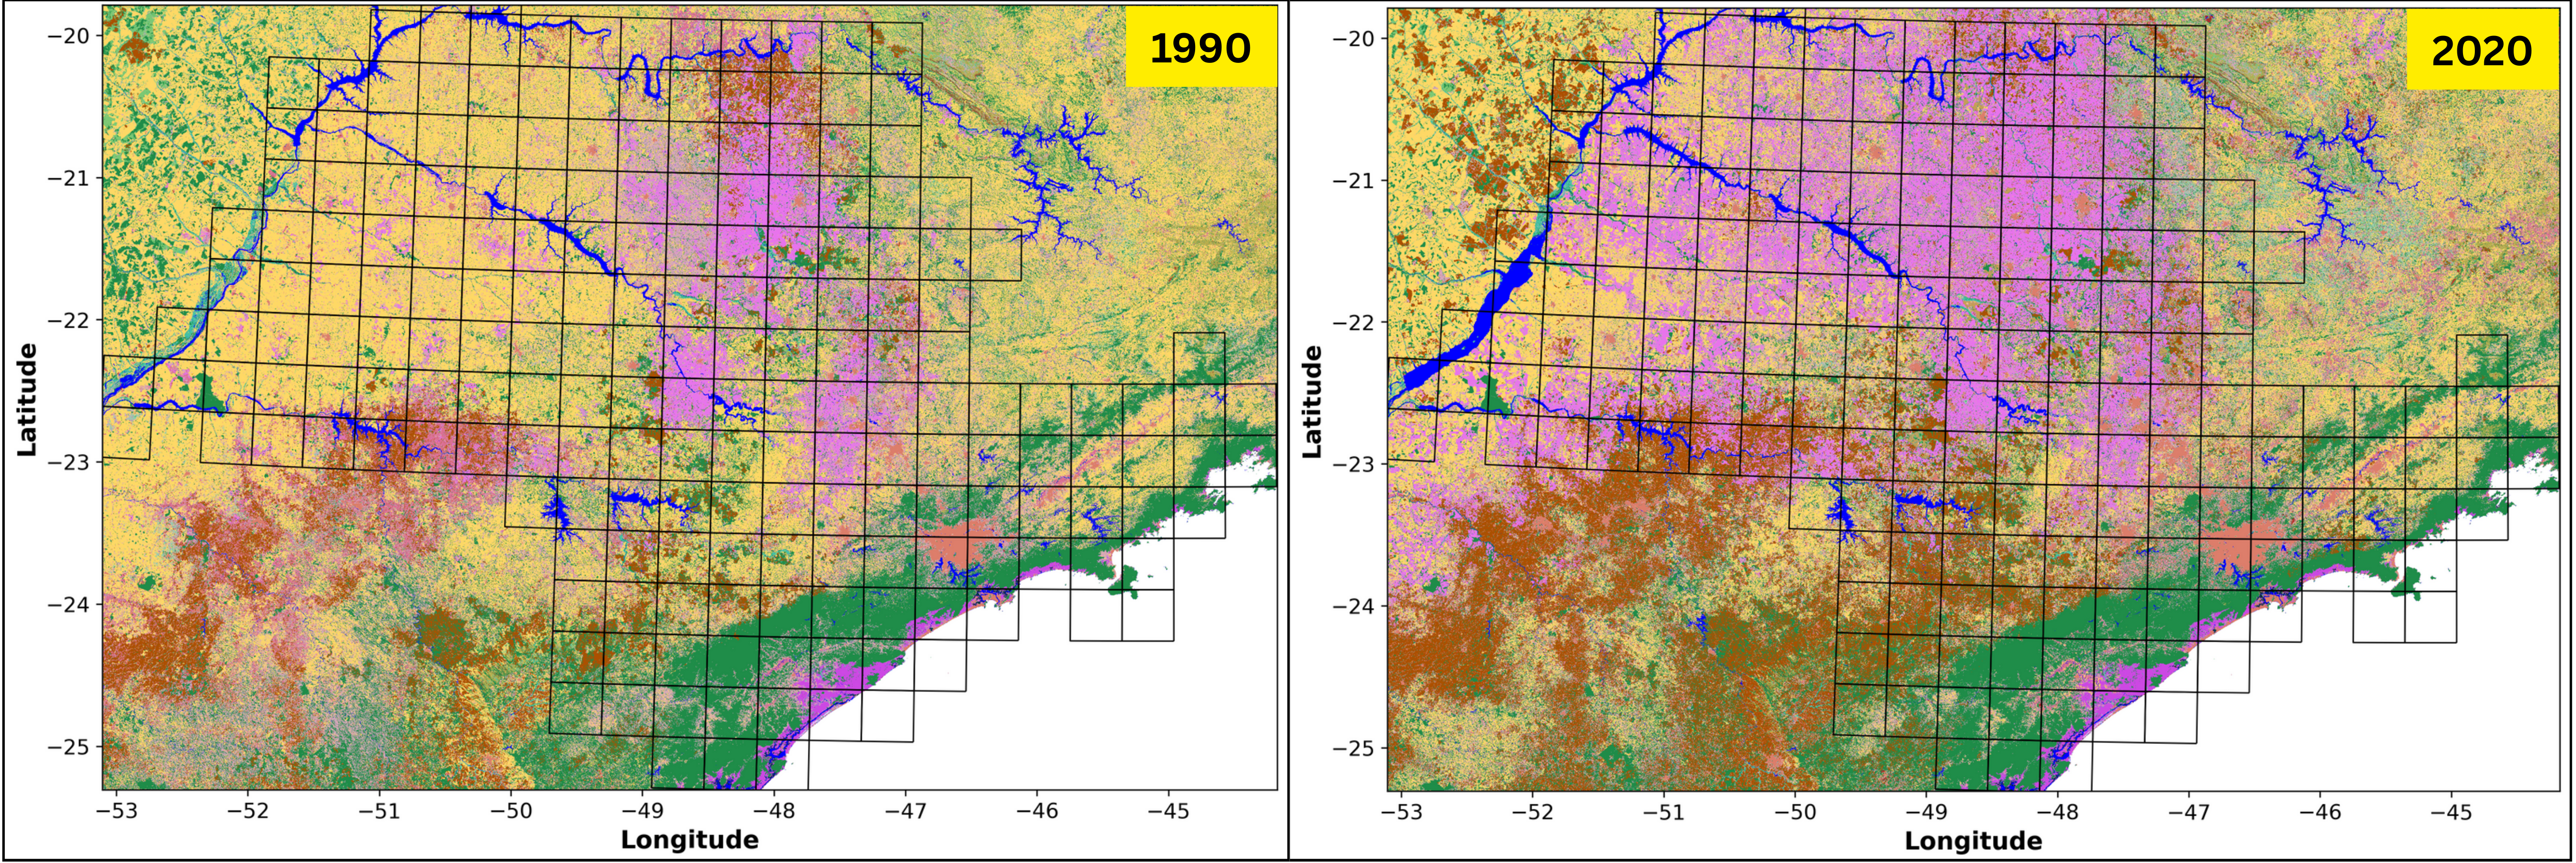
\includegraphics[width=1\textwidth]{mapa_grade_sp.png}
	\caption[Uso e cobertura da terra no estado de São Paulo em 1990 segundo classificação MapBiomas, Collection 9]{Uso e cobertura da terra no estado de São Paulo em 1990 segundo classificação MapBiomas, Collection 9. Observe a dominância de pastagens (tons amarelados), presença significativa de agricultura (tons rosados) e remanescentes de vegetação nativa (tons verdes) principalmente na Serra do Mar e Serra da Mantiqueira. Já ao lado direito o que temos é a relação do uso de cobertura da terra em 2020 segundo classificação, intensificação agrícola com redução de pastagens, e recuperação parcial de vegetação nativa em algumas áreas protegidas.}
	\label{fig:mapbiomas_sp_1990}
\end{figure}

A Figura \ref{fig:mapbiomas_sp_1990} apresenta a distribuição espacial das classes de uso e cobertura da terra no estado de São Paulo em dois momentos distintos (1990 e 2020), evidenciando transformações substanciais ao longo do período de três décadas. Em 1990, o território paulista apresentava configuração caracterizada pela dominância de pastagens (tons amarelados) ocupando extensas áreas nas regiões centro, oeste e noroeste do estado, intercaladas com agricultura intensiva (tons rosados), particularmente concentrada no norte e noroeste. As formações florestais nativas (tons verdes escuros) encontravam-se predominantemente preservadas na Serra do Mar (faixa costeira sudeste) e em remanescentes dispersos na Serra da Mantiqueira (extremo leste). As áreas urbanizadas (tons avermelhados) já apresentavam expressão significativa na região metropolitana de São Paulo e em cidades médias do interior.

Já em 2020 o que se revela são transformações marcantes nesta configuração. Observa-se intensificação agrícola substancial, com expansão de cultivos de cana-de-açúcar (tons rosa-lilás) nas regiões norte, noroeste e centro-oeste, ocupando áreas anteriormente destinadas a pastagens. A conversão de pastagens de baixa produtividade em agricultura mecanizada é particularmente evidente nas regiões de Ribeirão Preto, Barretos e Araçatuba. Simultaneamente, as formações florestais na Serra do Mar e Serra da Mantiqueira apresentam aparente expansão ou adensamento (tons verdes mais intensos). A mancha urbana apresenta expansão moderada mas geograficamente concentrada, com crescimento mais visível na região metropolitana de São Paulo e no entorno de cidades médias do interior, representada pela intensificação dos tons avermelhados.

O estado do Rio Grande do Norte, por sua vez, apresenta transformações ainda mais dramáticas (Figura \ref{fig:mapbiomas_rn_1990}). As alterações observadas caracterizam um dos processos de conversão de vegetação nativa mais severos.

\begin{figure}[htbp]
	\centering
	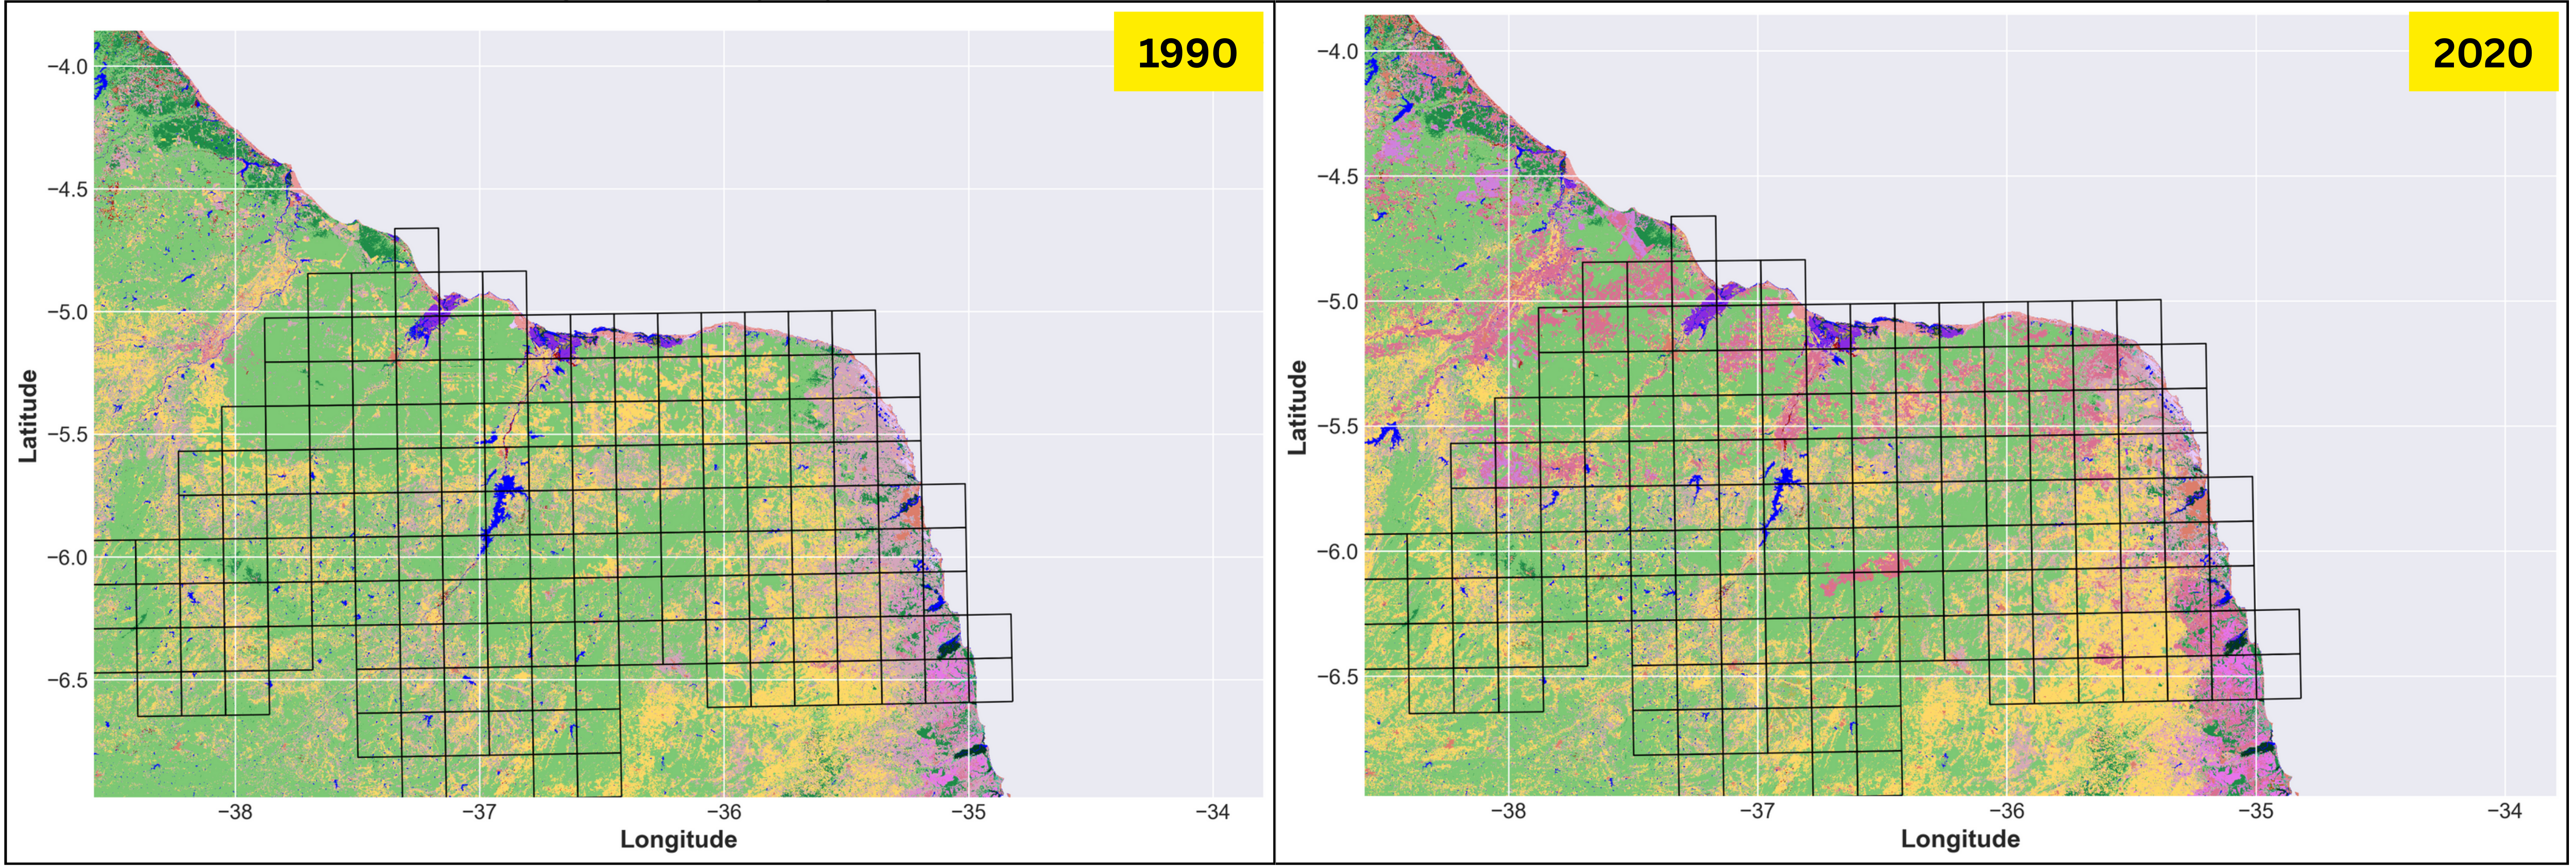
\includegraphics[width=1\textwidth]{mapa_grade_rn.png}
	\caption[Uso e cobertura da terra no estado do Rio Grande do Norte em 1990 segundo classificação MapBiomas, Collection 9]{Uso e cobertura da terra no estado do Rio Grande do Norte em 1990 segundo classificação MapBiomas, Collection 9. Observe a dominância de formação savânica (Caatinga) em tons verde-claro e verde-amarelado ocupando aproximadamente 79\% do território, refletindo extensão da vegetação nativa semiárida. A zona costeira apresenta manguezais (tons verde-escuro), aquicultura (tons lilás) e áreas urbanizadas. Já ao lado direito, em 2020, observa-se redução catastrófica da Caatinga (agora apenas 35,5\% do território), substituída principalmente por pastagens degradadas (tons amarelados), agricultura de sequeiro, solo exposto e áreas em diversos estágios de degradação ambiental.}
	\label{fig:mapbiomas_rn_1990}
\end{figure}

A Figura \ref{fig:mapbiomas_rn_1990} apresenta a distribuição espacial das classes de uso e cobertura da terra no Rio Grande do Norte em 1990 e 2020. Em 1990, o estado apresentava dominância de formação savânica (Caatinga) representada em tons verde-claro e verde-amarelado, cobrindo aproximadamente 79\% do território e distribuída de forma relativamente contínua pelas regiões central, sul e oeste. A vegetação de Caatinga preservada era particularmente expressiva nas regiões do Seridó (centro-sul) e no interior semiárido, intercalada com manchas de pastagem (tons amarelados) e agricultura de sequeiro. A zona costeira já apresentava maior heterogeneidade, com presença de áreas urbanizadas concentradas em Natal e outras cidades litorâneas (tons avermelhados), atividades de aquicultura incipientes (tons lilás), manguezais preservados (tons verde-escuro) e agricultura irrigada em áreas específicas do litoral leste. Formações campestres e campos alagados (tons alaranjados e ciano) eram visíveis em áreas de transição ecológica e várzeas.

O painel de 2020 apresenta uma transformação particularmente drástica desta configuração original. A cobertura de Caatinga sofreu redução significativa e espacialmente generalizada, com conversão massiva em pastagens degradadas (tons amarelados agora predominantes em vastas áreas do interior), agricultura de sequeiro de baixa produtividade, solo exposto e áreas em diversos estágios de degradação ambiental. Esta conversão é particularmente severa e visualmente impactante nas regiões centro-norte e central do estado, onde a vegetação nativa característica (tons verdes) foi substituída quase completamente por tons amarelados. Os remanescentes de Caatinga preservada (tons verdes) restringem-se a fragmentos dispersos e áreas específicas no sul do estado e em localidades pontuais. A região costeira apresenta expansão visível de áreas urbanizadas, especialmente em Natal, Mossoró e ao longo do litoral oriental (intensificação dos tons avermelhados), intensificação marcante da aquicultura com ampliação de manchas lilás. O contraste visual entre os dois painéis é extremamente marcante: o que em 1990 era um estado predominantemente coberto por vegetação nativa semiárida (tons verdes ocupando a maior parte do território) transformou-se em 2020 em território dominado por usos antrópicos de baixa produtividade e cobertura vegetal severamente degradada (tons amarelados).

\subsection{Avaliação e extremos de cobertura de solo no estado de São Paulo}

\begin{figure}[htbp]
	\centering
	\includegraphics[width=1\textwidth]{mapa_blocos_extremos_sp.png}
	\caption[Áreas de maior e menor mudança de formação florestal em percentis]{Áreas de maior e menor mudança de formação florestal em percentis, onde a maior perda (desmatamento) está em destaque com tons avermelhados, a menor perda ou cobertura constante em tons amarelados, já o ganho de área florestal está representada em tons de verde.}
	\label{fig:mapa_blocos_extremos_sp}
\end{figure}

Ao analisar a Figura \ref{fig:mapa_blocos_extremos_sp} o que se destacam são: A evolução temporal da cobertura de formação florestal (predominantemente Mata Atlântica) apresenta duas trajetórias distintas que refletem diferentes contextos espaciais. Em áreas sob maior pressão de conversão agrícola e urbana, a cobertura florestal reduziu-se de 15,0\% em 1990 para 6,0\% em 2020, representando perda absoluta de 9,0 pontos percentuais. Avaliando progressivamente o comportamento de 10 em 10 anos, o que se observa é uma queda progressiva nos últimos anos, estabilizando-se de 2010 à 2020, Figura \ref{fig:evolucao_cobertura_sp}.

\begin{figure}[htbp]
	\centering
	\includegraphics[width=\textwidth]{evolucao_cobertura_vegetal_sp.png}
	\caption{Evolução temporal da cobertura de formação florestal no estado de São Paulo (1990-2020).}
	\label{fig:evolucao_cobertura_sp}
\end{figure}


Em contraste, a linha verde representa áreas com trajetória oposta, iniciando em 40,3\% de cobertura florestal em 1990 e apresentando crescimento progressivo para 45,0\% (2000), 47,0\% (2010) e 49,8\% (2020), totalizando ganho de 9,5 pontos percentuais ao longo do período.

A análise integrada das duas figuras evidencia portanto que as mudanças na cobertura florestal paulista não seguem padrão estadual homogêneo. As perdas concentram-se em regiões de agricultura intensiva no interior (noroeste), enquanto ganhos ocorrem em áreas de proteção ambiental e topografia acidentada (Serra do Mar).

\subsubsection*{Análises complementares}
As pastagens, que em 1990 ocupavam aproximadamente $57,4\%$ do território estadual, reduziram-se para apenas $7,8\%$ em 2020{,}. Esta redução massiva reflete múltiplos processos: conversão de pastagens degradadas de baixa produtividade em agricultura intensiva mecanizada (principalmente cana-de-açúcar, citros e grãos); abandono de pastagens marginalmente produtivas em áreas de topografia acidentada com subsequente regeneração natural da vegetação; e em menor escala, reflorestamento comercial com eucalipto ou pinus.

\subsection{Avaliação e extremos de cobertura de solo no estado do Rio Grande do Norte}

A análise espacial (Figura \ref{fig:mapa_blocos_extremos_rn}) revela alta heterogeneidade, com células individuais apresentando perdas de até $-43{,}4\%$ e ganhos de até $+14{,}0\%$ de cobertura de Caatinga entre 1990 e 2020. O mapa evidencia padrão espacial complexo: áreas de maior perda (tons vermelho-escuro) concentram-se predominantemente na região centro-norte do estado (célula com perda máxima de $-43{,}4\%$ localizada em latitude $-5^\circ$ e longitude $-37^\circ$, correspondendo aproximadamente à região do Seridó), enquanto áreas de ganho ou menor mudança (tons verdes) distribuem-se principalmente no sul e sudoeste (célula com ganho máximo de $+14{,}0\%$ em latitude $-6{,}5^\circ$ e longitude $-38^\circ$). A região central e leste apresenta mosaico heterogêneo de perdas moderadas a severas (tons alaranjados a vermelhos).

\begin{figure}[htbp]
	\centering
	\includegraphics[width=\textwidth]{mapa_blocos_extremos_rn.png}
	\caption[Distribuição espacial das mudanças na cobertura de formação savânica (Caatinga) no Rio Grande do Norte (1990-2020)]{Distribuição espacial das mudanças na cobertura de formação savânica (Caatinga) no Rio Grande do Norte (1990-2020) por célula de 100×100 km. Tons vermelhos indicam maior perda (desmatamento); tons amarelados representam mudanças moderadas; tons verdes indicam ganho ou estabilidade.}
	\label{fig:mapa_blocos_extremos_rn}
\end{figure}

A Figura \ref{fig:evolucao_cobertura_rn} revela as trajetórias temporais que caracterizam estas regiões extremas. A linha vermelha representa áreas sob maior pressão antrópica, onde a cobertura de Caatinga sofreu redução de 79,0\% em 1990 para aproximadamente 68,0\% em 2000, seguida por nova queda para 60,0\% em 2010, decaindo progressivamente para 35,5\% em 2020. Esta trajetória evidencia processo de degradação acelerada, particularmente severa na última década (2010-2020), quando ocorreu a maior taxa absoluta de perda ($-24{,}5\%$ em apenas 10 anos).

\begin{figure}[htbp]
	\centering
	\includegraphics[width=\textwidth]{evolucao_cobertura_vegetal_rn.png}
	\caption[Evolução temporal da cobertura de formação savânica (Caatinga) no Rio Grande do Norte (1990-2020)]{Evolução temporal da cobertura de formação savânica (Caatinga) no Rio Grande do Norte (1990-2020). Linha vermelha representa células com maior perda de cobertura; linha verde representa células com menor mudança ou recuperação.}
	\label{fig:evolucao_cobertura_rn}
\end{figure}

Em contraste marcante, a linha verde representa áreas com trajetória de recuperação ou preservação relativa, iniciando em 56,6\% de cobertura em 1990 e apresentando crescimento progressivo para 62,0\% (2000), 73,0\% (2010), com leve redução para 70,6\% (2020), resultando em ganho de 14{,}0\% ao longo do período. Passando para o processo de diminuição, linhas vermelha, é observado um decaimento considerável da perda savânica após 2010 (linha vermelha: queda de 60\% para 35,5\%) contrasta com relativa estabilização nas áreas menos degradadas (linha verde: pequena redução de 73\% para 70,6\%).

A análise integrada das duas figuras evidencia que o Rio Grande do Norte experimenta processo de diferenciação espacial extrema, com áreas apresentando um comportamento e recuperação de cobertura vegetal, enquanto a maioria do território sofre degradação progressiva quando observado em conjunto com a Figura \ref{fig:mapa_blocos_extremos_rn} que demonstra uma mudança considerável nos dois cenários.

% ANÁLISE DAS VARIÁVEIS CLIMÁTICAS NOS EXTREMOS DE MUDANÇA DE COBERTURA VEGETAL

\section{Variáveis climáticas em áreas de extremos de mudança de cobertura}

A análise das variáveis climáticas em células de grade apresentadas no decorrer desta seção pelas Figuras \ref{fig:mapa_blocos_extremos_sp} e \ref{fig:mapa_blocos_extremos_sp} com a descrição das localidades das mudanças extremas de mudança de cobertura vegetal, permite avaliar se as variações de cobertura estão associados aos padrões climáticos analisados nas seções anteriores. Para cada estado, selecionaram-se células representando os extremos: células com maior perda de vegetação nativa versus células com menor perda ou ganho de vegetação. As médias anuais de temperatura e radiação solar e acumulados de precipitação foram calculadas para estes dois grupos ao longo do período 1990-2020.

\subsection{São Paulo: Formação Florestal}

\subsubsection*{Temperatura}

A Figura \ref{fig:temp_extremos_sp} apresenta as médias anuais de temperatura para células com maior versus menor redução de formação florestal no estado de São Paulo. Observa-se diferença térmica e persistente ao longo de todo o período analisado. Células com maior redução de vegetação florestal (linha vermelha) apresentam temperaturas consistentemente elevadas, oscilando entre 24,0 e 26,5 °C ao longo da série temporal, com média aproximada de 24,8 °C. Em contraste, células com menor redução ou ganho florestal (linha verde) mantêm-se consistentemente mais frias, variando entre 19,0 e 20,5 °C, com média próxima a 19,5 °C.

\begin{figure}[htbp]
	\centering
	\includegraphics[width=\textwidth]{medias_anuais_temp_celsius_formacao_florestal_sp.png}
	\caption{Médias anuais de temperatura (°C) em células com maior versus menor redução de formação florestal em São Paulo (1990-2020).}
	\label{fig:temp_extremos_sp}
\end{figure}

A diferença entre os dois grupos mantém-se notavelmente constante em aproximadamente 5,0 a 5,5 °C ao longo de três décadas. Esta magnitude e persistência sugerem que a diferença de temperatura é primariamente determinada por fatores geográficos estruturais (altitude, latitude) ao invés de mudanças dinâmicas na cobertura vegetal. As células com maior perda florestal localizam-se predominantemente no interior noroeste do estado, em altitudes baixas (300-500 m) e latitudes menores, enquanto células com menor perda ou ganho concentram-se na Serra do Mar, em altitudes elevadas (800-1200 m) e latitude ligeiramente maior.

Ambos os grupos apresentam tendência de aquecimento ao longo do período, particularmente visível após 2010. Células com maior perda florestal mostram aquecimento de aproximadamente 1,5 a 2,0 °C entre 1990 e 2020, enquanto células preservadas apresentam aquecimento de magnitude similar (1,0 a 1,5 °C).

\subsubsection*{Radiação Solar}

A Figura \ref{fig:rad_extremos_sp} descreve o comportamento de radiação solar incidente fundamentalmente distinto entre os dois grupos de células. A célula com maior perda florestal (linha vermelha) apresentam valores consistentemente elevados, oscilando entre 205 e 235 W/m$^2$ ao longo da série temporal, com média aproximada de 220 W/m$^2$. Células preservadas (linha verde) mantêm radiação substancialmente inferior, variando entre 160 e 197 W/m$^2$, com média próxima a 180 W/m$^2$.

\begin{figure}[htbp]
	\centering
	\includegraphics[width=\textwidth]{medias_anuais_SIS_formacao_florestal_sp.png}
	\caption{Médias anuais de radiação solar incidente (W/m$^2$) em células com maior versus menor redução de formação florestal em São Paulo (1990-2020).}
	\label{fig:rad_extremos_sp}
\end{figure}

A diferença radiativa entre os grupos permanece aproximadamente constante em 40 a 50 W/m$^2$ ao longo do período, representando redução de cerca de 20 a 25\% na radiação disponível nas áreas preservadas comparadas às áreas desmatadas. Esta diferença é geograficamente determinada: células preservadas na Serra do Mar apresentam maior nebulosidade orográfica devido ao levantamento de massas de ar úmidas oceânicas, enquanto células do interior noroeste beneficiam-se de maior transparência atmosférica e menor nebulosidade média o que implica em maior incidência de radiação sobre a superfície.

Ambos os grupos apresentam tendência de aumento da radiação solar ao longo do período, particularmente evidente após 2010. A taxa de aumento é similar entre os grupos (aproximadamente 15 a 20 W/m$^2$ ao longo de 30 anos).

\subsubsection*{Precipitação}

A Figura \ref{fig:prec_extremos_sp} apresenta diferenças de acumulado de precipitação marcantes entre os dois grupos de células. Células com menor redução ou ganho florestal (linha verde), localizadas predominantemente na Serra do Mar, apresentam precipitação acumulada anual consistentemente superior, oscilando entre 80.000 e 110.000 mm acumulados (equivalente a aproximadamente 800 a 1100 mm anuais quando considerada a área total das células), com média próxima a 90.000 mm. Em contraste, células com maior perda florestal (linha vermelha), situadas no interior noroeste, apresentam valores substancialmente inferiores, variando entre 60.000 e 95.000 mm, com média próxima a 75.000 mm.

\begin{figure}[htbp]
	\centering
	\includegraphics[width=\textwidth]{acumulados_anuais_prec_formacao_florestal_sp.png}
	\caption[Precipitação total anual (mm) em células com maior versus menor redução de formação florestal em São Paulo (1990-2020)]{Precipitação total anual (mm) em células com maior versus menor redução de formação florestal em São Paulo (1990-2020). Valores representam acumulados totais considerando a área das células de grade.}
	\label{fig:prec_extremos_sp}
\end{figure}

A diferença de precipitação entre os grupos mantém-se relativamente constante ao longo do período, oscilando entre 10.000 e 25.000 mm dependendo do ano específico, equivalente a aproximadamente 15 a 30\% a mais de precipitação nas áreas preservadas. Esta diferença é primariamente determinada por efeitos orográficos: células preservadas na Serra do Mar beneficiam-se de intensificação pluviométrica devido ao levantamento forçado de massas de ar úmidas oceânicas que ascendem as encostas da serra, experimentam resfriamento adiabático, condensação e precipitação intensificada particularmente nas vertentes voltadas para o oceano.

A interpretação destas diferenças pluviométricas requer cuidado: embora células preservadas recebam substancialmente mais precipitação, esta diferença reflete primariamente localização geográfica (Serra do Mar versus interior) ao invés de efeitos diretos da cobertura vegetal. As mesmas características topográficas que induzem alta precipitação orográfica também favoreceram historicamente a preservação florestal, criando correlação geográfica que não implica necessariamente causalidade. Efeitos da vegetação sobre precipitação local (através de evapotranspiração e reciclagem de umidade) podem existir mas são secundários comparados ao forte controle topográfico dominante.

\subsection{Rio Grande do Norte: Formação Savânica}

\subsubsection*{Temperatura}

A Figura \ref{fig:temp_extremos_rn} apresenta as médias anuais de temperatura para células com maior versus menor redução de Caatinga no Rio Grande do Norte. Em contraste marcante com São Paulo, observa-se que os dois grupos apresentam temperaturas surpreendentemente similares ao longo de todo o período analisado. Células com maior redução de Caatinga (linha vermelha) oscilam entre 27,0 e 28,6 °C, enquanto células com menor redução ou ganho (linha verde) variam entre 26,4 e 28,6 °C, com as duas linhas frequentemente convergindo ou até invertendo suas posições relativas.

\begin{figure}[htbp]
	\centering
	\includegraphics[width=\textwidth]{temp.png}
	\caption{Médias anuais de temperatura (°C) em células com maior versus menor redução de formação savânica (Caatinga) no Rio Grande do Norte (1990-2020).}
	\label{fig:temp_extremos_rn}
\end{figure}

A diferença térmica média entre os grupos é mínima, tipicamente inferior a 0,5 °C, e não apresenta consistência temporal ou espacial. Ambos os grupos apresentam alta variabilidade interanual (oscilações de até 2 °C entre anos consecutivos), refletindo flutuações em circulação atmosférica e nebulosidade. Esta variabilidade supera amplamente qualquer possível diferença sistemática entre áreas preservadas e degradadas, dificultando severamente a identificação de sinais associados especificamente a mudanças na cobertura de Caatinga. A análise visual sugere possível tendência sutil de aquecimento ao longo do período em ambos os grupos, consistente com tendências regionais apresentadas anteriormente, mas sem diferença detectável nas taxas de aquecimento entre células preservadas e degradadas.

\subsubsection*{Radiação Solar}

A Figura \ref{fig:rad_extremos_rn} apresenta padrão notavelmente distinto daquele observado em São Paulo. Células com maior redução de Caatinga (linha vermelha) e células com menor redução ou ganho (linha verde) apresentam valores de radiação solar surpreendentemente similares, oscilando em faixas que se sobrepõem substancialmente ao longo da série temporal. Ambos os grupos variam entre aproximadamente 245 e 278 W/m$^2$, com alta variabilidade interanual mas sem diferença sistemática consistente entre eles.

\begin{figure}[htbp]
	\centering
	\includegraphics[width=\textwidth]{rad.png}
	\caption{Médias anuais de radiação solar incidente (W/m$^2$) em células com maior versus menor redução de formação savânica (Caatinga) no Rio Grande do Norte (1990-2020).}
	\label{fig:rad_extremos_rn}
\end{figure}

A alta variabilidade interanual observada em ambos os grupos (oscilações de até 30 a 35 W/m$^2$ entre anos consecutivos) supera amplamente qualquer diferença média entre os grupos, dificultando a identificação de sinais associados especificamente a mudanças na cobertura vegetal. Esta variabilidade está provavelmente associada a flutuações na nebulosidade durante a estação chuvosa, que varia dramaticamente de ano para ano dependendo da intensidade e posicionamento da Zona de Convergência Intertropical.

\subsubsection*{Precipitação}

A Figura \ref{fig:prec_extremos_rn} apresenta o comportamento da precipitação acumulada com características específicas do semiárido. Ambos os grupos (maior redução - linha vermelha; menor redução ou ganho - linha verde) apresentam precipitação total anual variando entre 200 e 1250 mm, com variabilidade interanual extremamente elevada que domina completamente qualquer diferença média entre os grupos.

\begin{figure}[htbp]
	\centering
	\includegraphics[width=\textwidth]{prec.png}
	\caption{Precipitação total anual (mm) em células com maior versus menor redução de formação savânica (Caatinga) no Rio Grande do Norte (1990-2020).}
	\label{fig:prec_extremos_rn}
\end{figure}

O coeficiente de variação interanual para ambos os grupos excede 60\%, valor extremamente elevado mesmo para padrões semiáridos. Eventos de seca severa (precipitação <300 mm/ano) alternam-se com anos relativamente úmidos ($>$1000 mm/ano) sem padrão previsível. Esta alta variabilidade dificulta a identificação de possíveis diferenças entre áreas preservadas e degradadas.

Células com menor redução ou ganho de Caatinga (linha verde) apresentam tendência sutil de precipitação ligeiramente superior em alguns anos, particularmente visível nos picos de 2008-2009 (~1250 mm) e 2024 (~1150 mm). No entanto, esta diferença não é consistente ao longo da série e pode refletir simplesmente localização geográfica das células (sul do estado tipicamente recebe precipitação ligeiramente superior) ao invés de efeitos diretos da cobertura vegetal.

\subsection{Evolução espaciotemporal das variáveis climáticas e uso da terra}

As Figuras \ref{fig:mapas_temporais_rn} e \ref{fig:mapas_temporais_sp} apresentam a evolução espacial simultânea de uso da terra e variáveis climáticas em intervalos decadais (1990, 2000, 2010, 2020), permitindo avaliação visual de possíveis associações entre transformações de cobertura vegetal e mudanças climáticas localizadas.


\subsubsection*{São Paulo}

\begin{figure}[H]
	\centering
	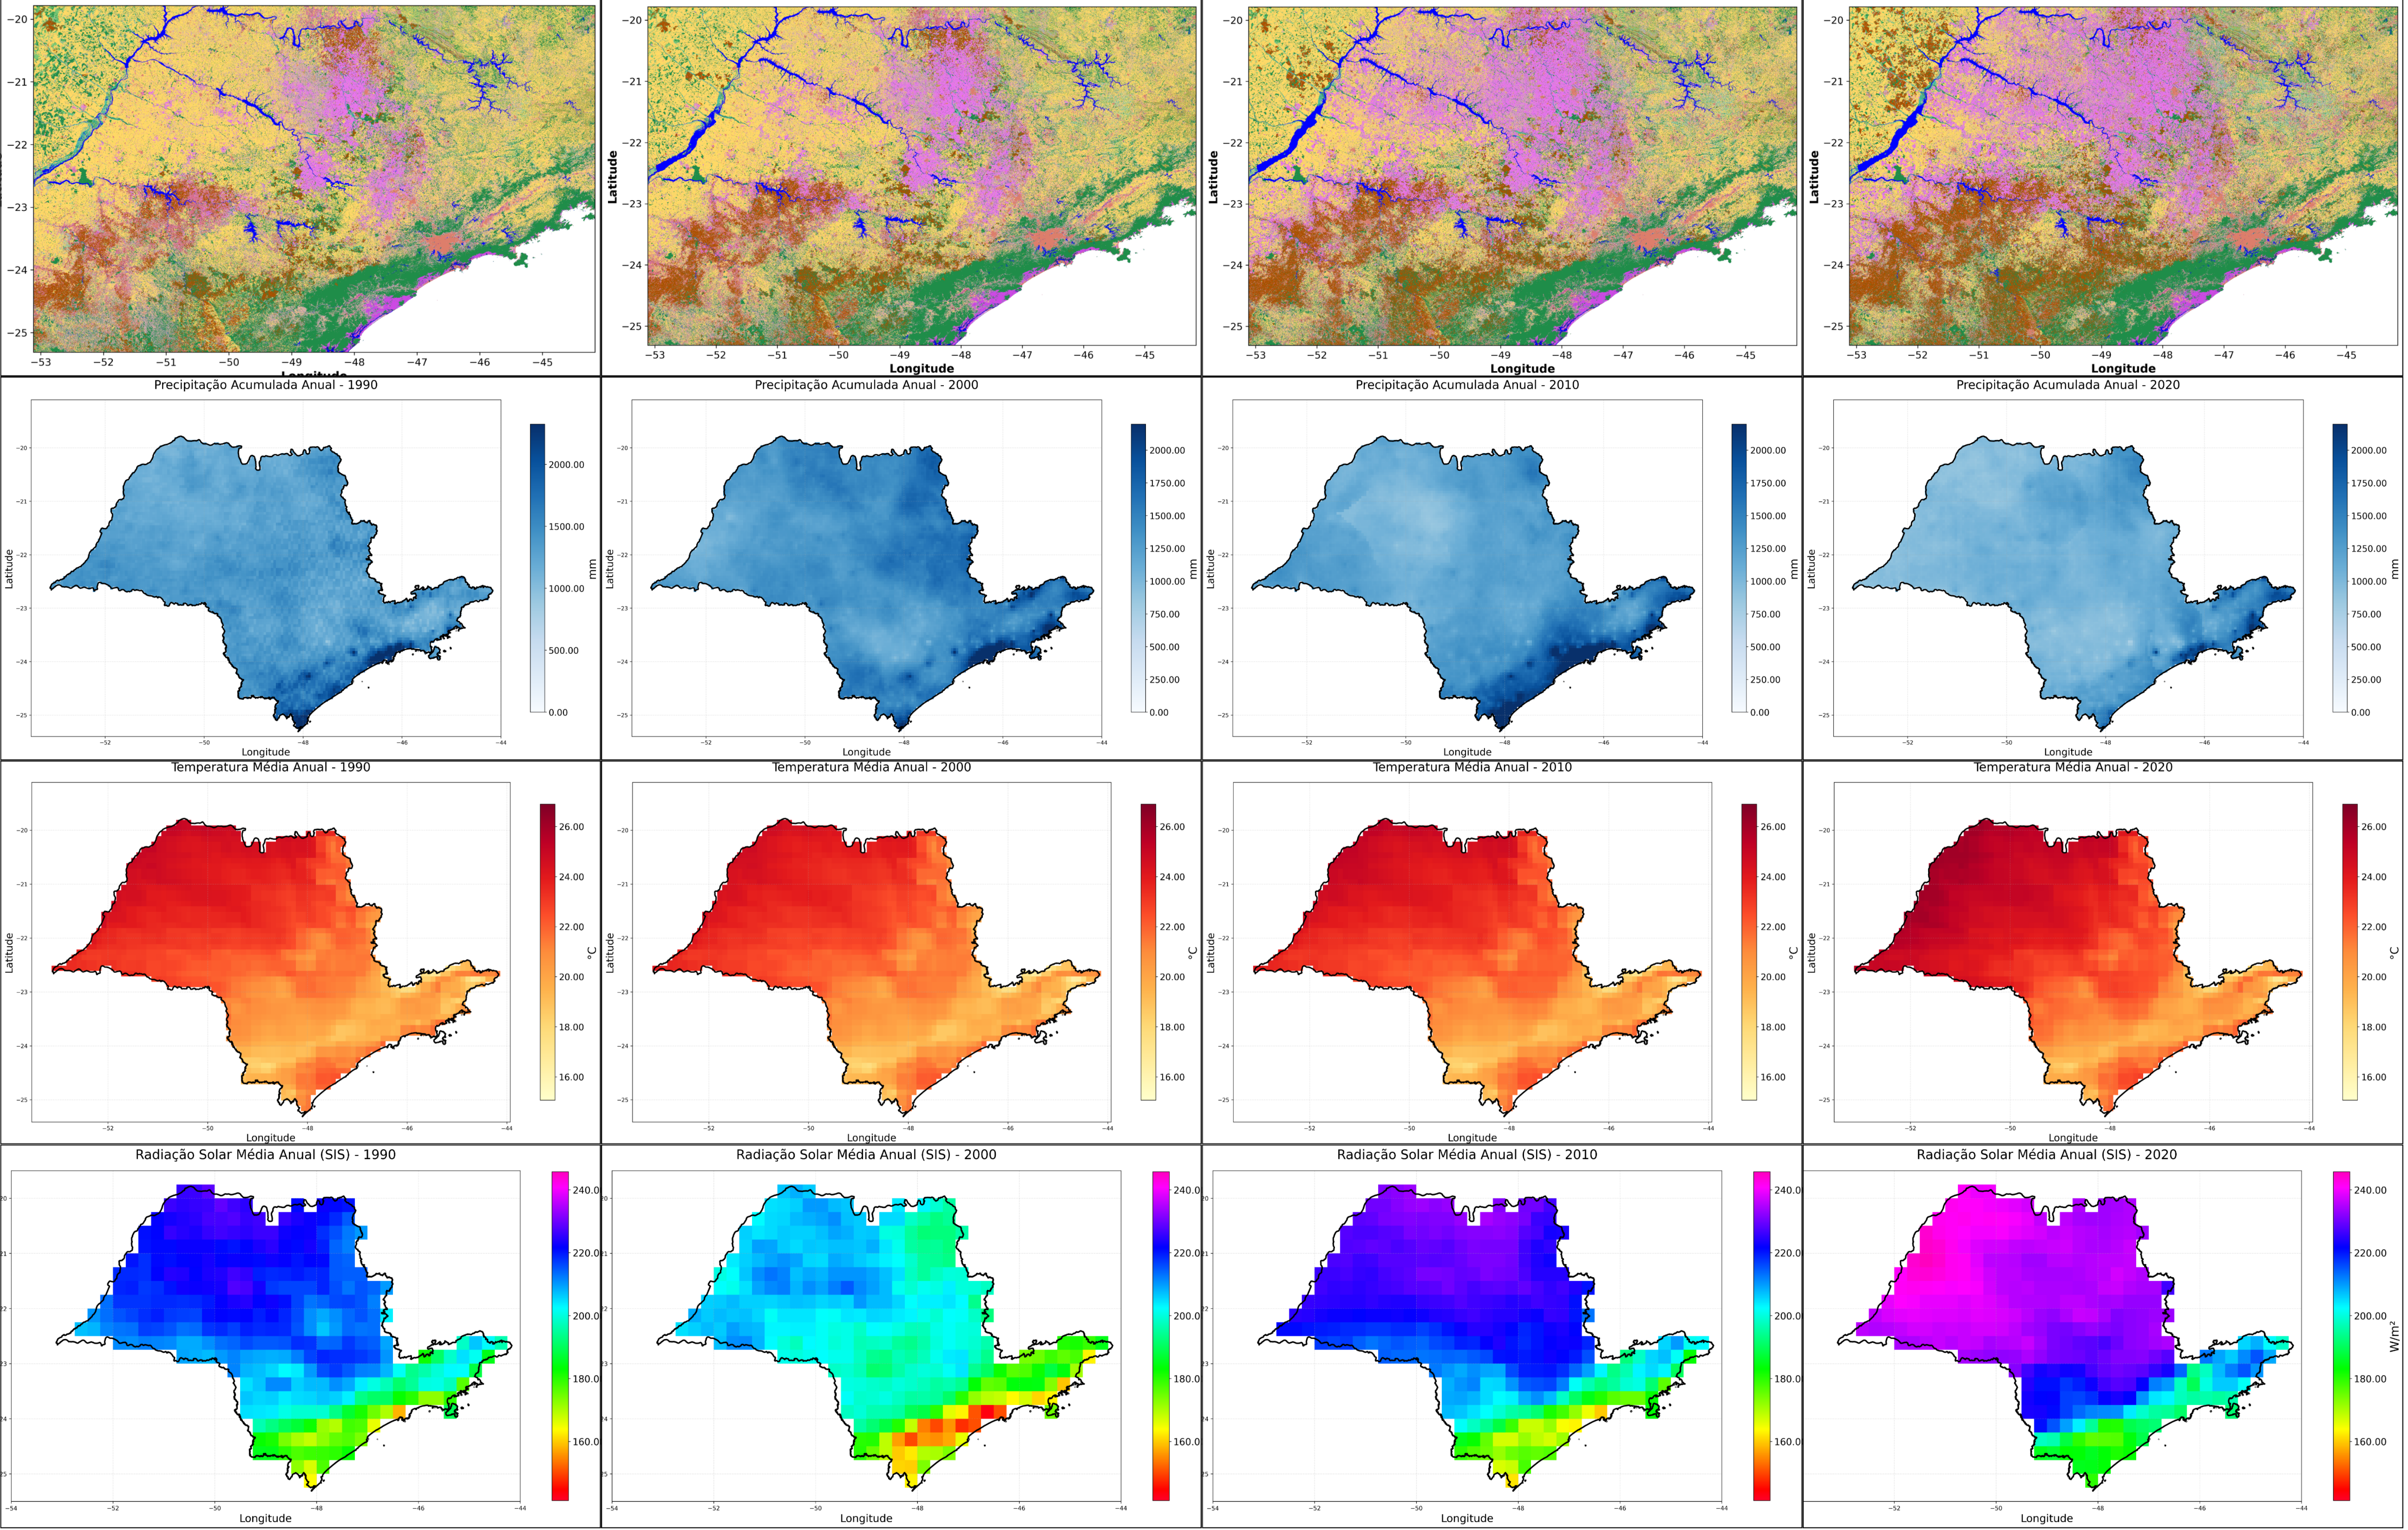
\includegraphics[width=\textwidth]{mapas_sp.png}
	\caption[Evolução temporal do uso da terra - SP]{Evolução temporal do uso da terra (linha superior), precipitação acumulada anual (segunda linha), temperatura média anual (terceira linha) e radiação solar média anual (linha inferior) em São Paulo para os anos de 1990, 2000, 2010 e 2020.}
	\label{fig:mapas_temporais_sp}
\end{figure}

A linha superior da Figura \ref{fig:mapas_temporais_sp} descreve a transformação agrícola progressiva. Entre 1990 e 2020, observa-se conversão substancial de pastagens (tons amarelados) em agricultura intensiva (tons rosa-lilás) nas regiões norte, noroeste e central do estado. Simultaneamente, a Serra do Mar mantém ou intensifica tonalidade verde, consistente com preservação ou recuperação de cobertura florestal.

As variáveis climáticas (linhas 2-4) mantêm padrões espaciais notavelmente estáveis ao longo dos 30 anos. A precipitação preserva gradiente litoral-interior característico em todos os períodos. A temperatura mostra gradiente topográfico estável (Serra do Mar mais fria, interior mais quente) que se mantém praticamente inalterado apesar das transformações de uso da terra.

A radiação solar mantém padrão inverso ao da precipitação (máximos no interior, mínimos no litoral) de forma consistente nos quatro períodos. A estabilidade deste padrão ao longo de três décadas de intensas mudanças agrícolas sugere que nebulosidade, determinada primariamente por topografia e circulação atmosférica de grande escala, domina sobre possíveis efeitos da vegetação sobre radiação.

\subsubsection*{Rio Grande do Norte}

\begin{figure}[H]
	\centering
	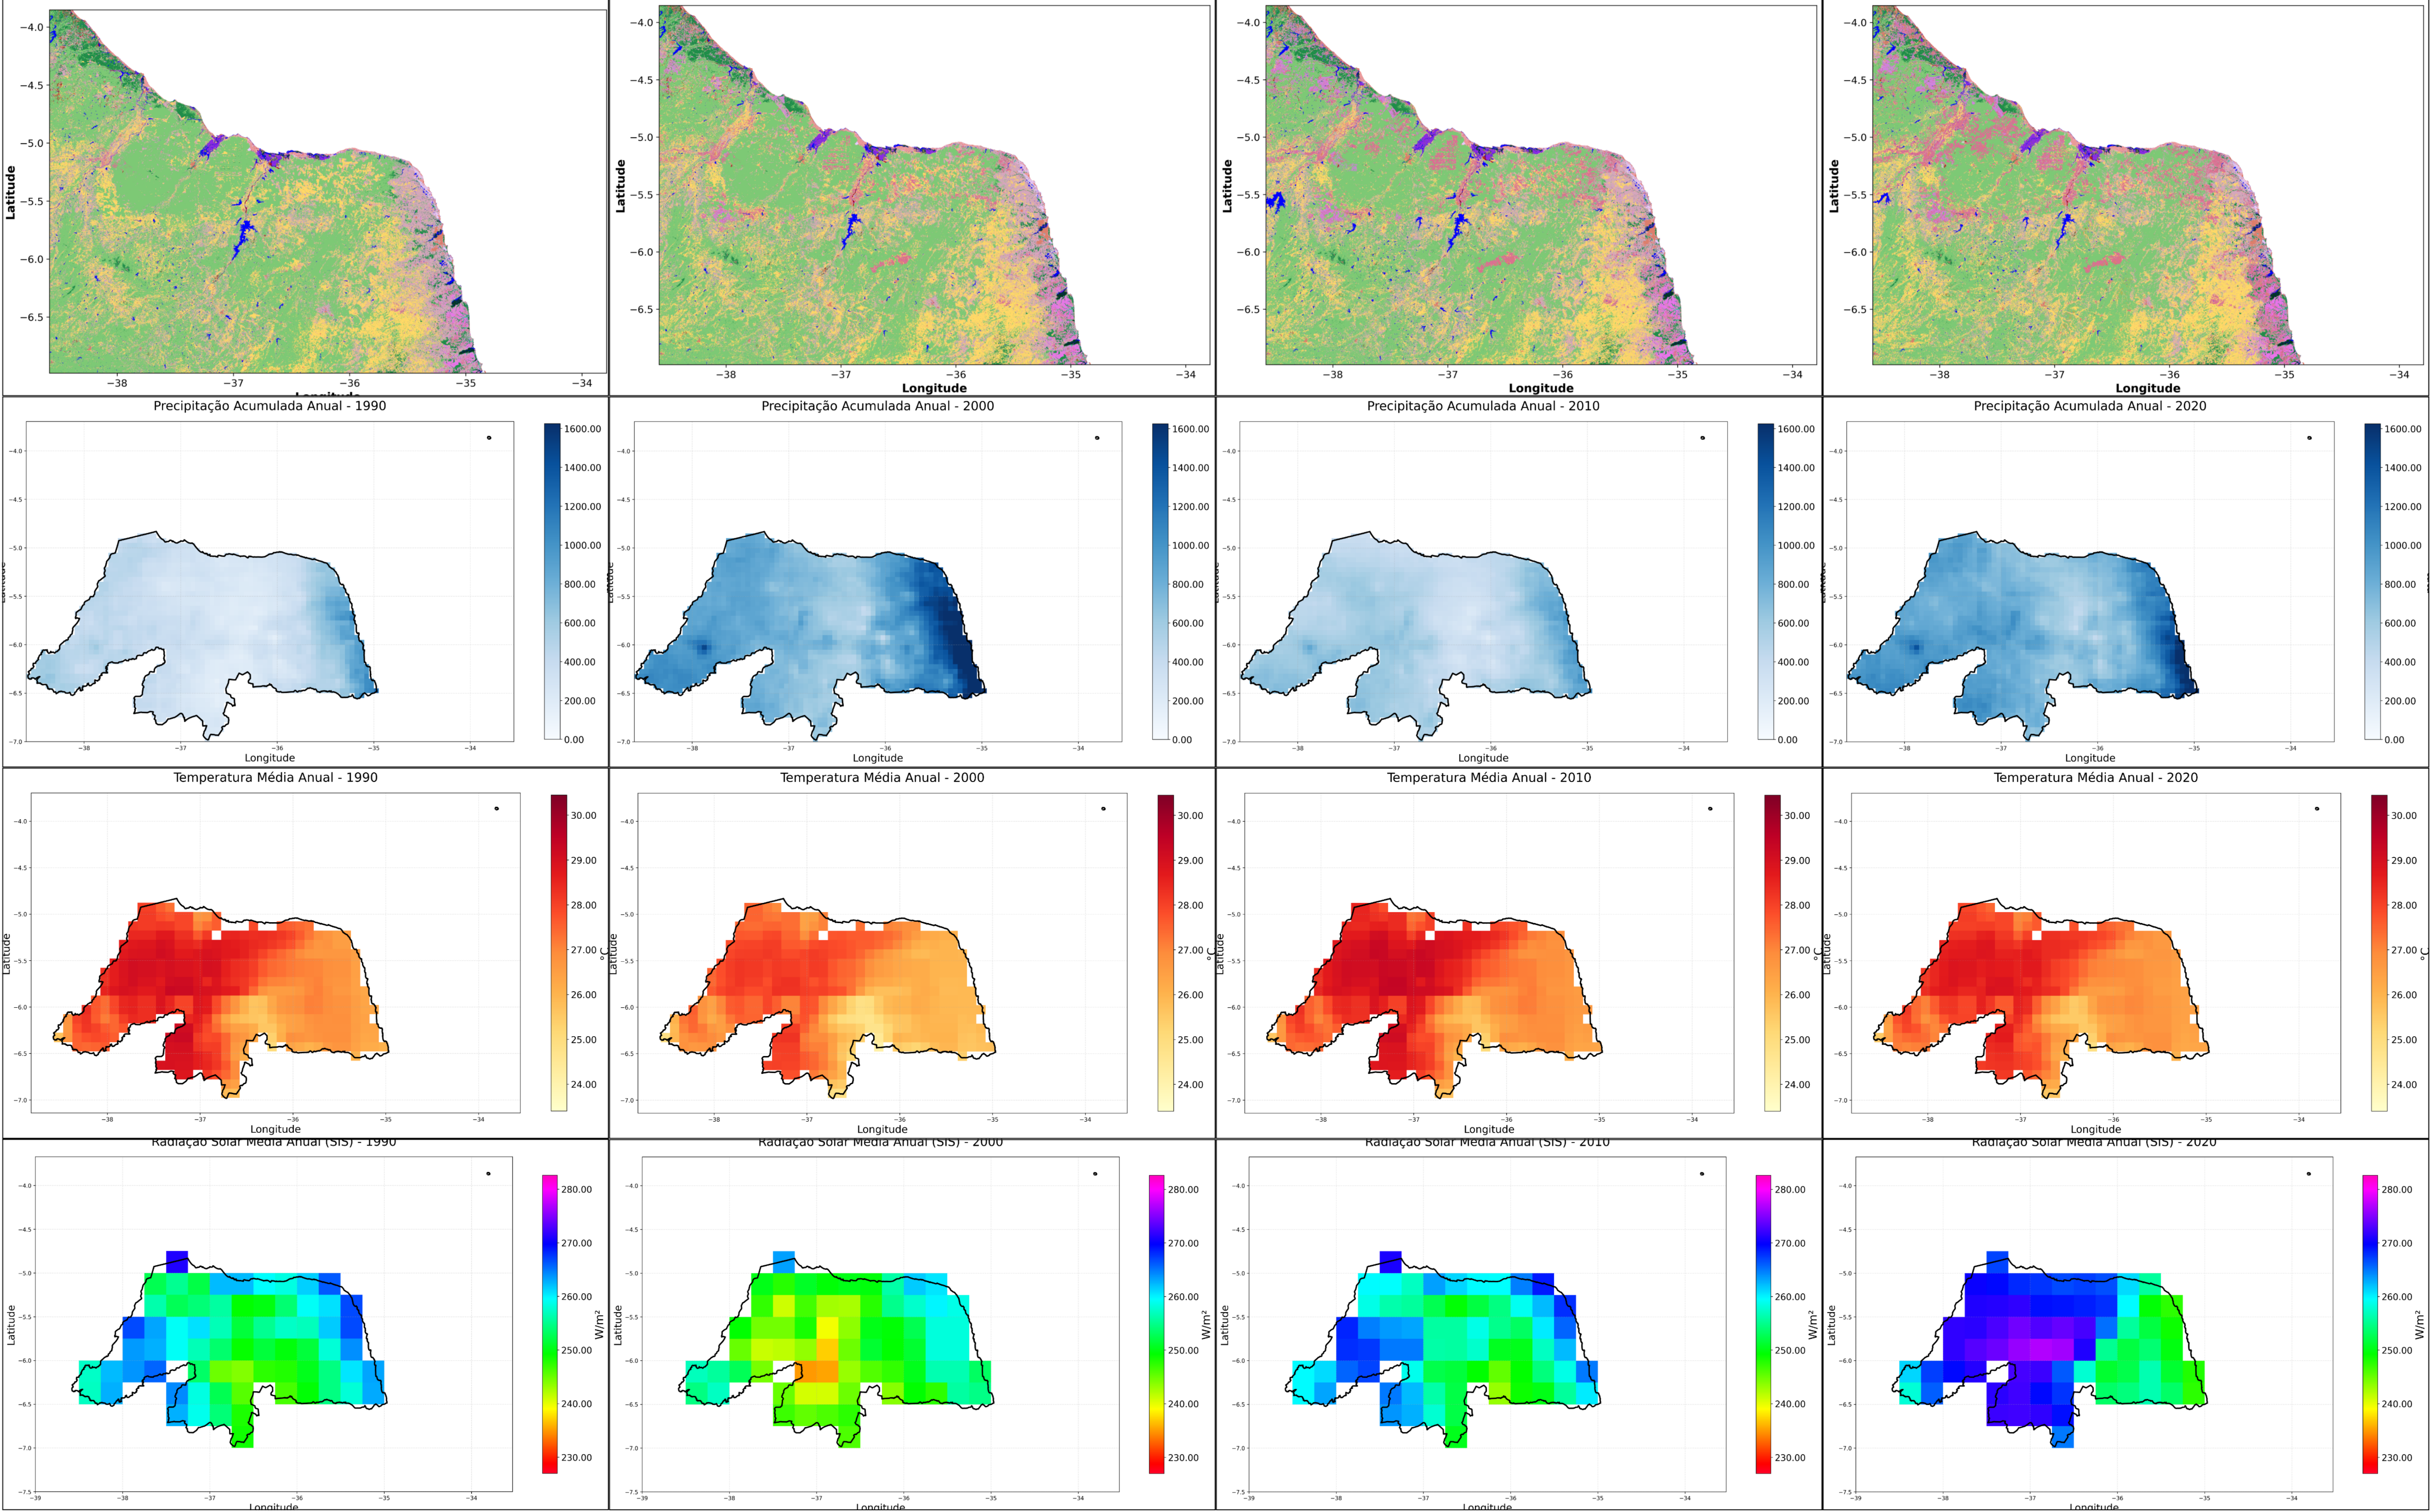
\includegraphics[width=\textwidth]{mapas_rn.png}
	\caption[Evolução temporal do uso da terra - RN]{Evolução temporal do uso da terra (linha superior), precipitação acumulada anual (segunda linha), temperatura média anual (terceira linha) e radiação solar média anual (linha inferior) no Rio Grande do Norte para os anos de 1990, 2000, 2010 e 2020.}
	\label{fig:mapas_temporais_rn}
\end{figure}

A linha superior da Figura \ref{fig:mapas_temporais_rn} apresenta o processo de degradação progressiva e espacialmente heterogênea da Caatinga. Entre 1990 e 2020, observa-se conversão substancial de áreas verdes (Caatinga preservada) em tons amarelados e acastanhados (pastagens degradadas, solo exposto), particularmente intensa nas regiões centro-norte e central do estado.

As linhas de precipitação (segunda linha) e temperatura (terceira linha) não apresentam padrões espaciais de mudança claramente associados às áreas de maior degradação de Caatinga. A precipitação mantém gradiente leste-oeste característico (litoral úmido, interior seco) em todos os quatro períodos, com variações interanuais que refletem primariamente flutuações na intensidade da estação chuvosa ao invés de mudanças sistemáticas associadas a uso da terra.

A temperatura mostra gradiente norte-sul relativamente estável ao longo do período, com interior norte mais quente (27-28 °C) e litoral sul ligeiramente mais frio (26-27 °C). Não se identifica visualmente aquecimento localizado consistente em áreas que experimentaram maior degradação.

A radiação solar apresenta padrão espacial complexo que varia substancialmente entre os anos analisados, refletindo primariamente flutuações na nebulosidade durante a estação chuvosa. Não se observa aumento sistemático de radiação em áreas de maior degradação.


\section{Avaliação quantitativa sobre a influência da cobertura de superfície sobre variáveis climáticas}

Tomando como base os resultados anteriores que não evidenciavam claramente a influência da cobertura de superfície sobre as variáveis climáticas analisadas, adotou-se abordagem quantitativa mais refinada para investigar a relação entre diferentes tipos de cobertura da terra e as variáveis climáticas temperatura do ar, precipitação acumulada e radiação solar incidente na superfície. Esta análise considerou quatro classes distintas de cobertura segundo a classificação MapBiomas: Formação Florestal (Classe 3) para São Paulo, Formação Savânica (Classe 4) para Rio Grande do Norte, e Área Urbanizada (Classe 24) para ambos os estados, permitindo avaliar tanto o papel da vegetação nativa quanto o impacto da urbanização sobre o clima local.

A fundamentação teórica desta análise baseia-se no entendimento de que as modificações na cobertura da terra alteram o balanço de energia superficial através de múltiplos mecanismos biofísicos \citep{oke1982energetic}. A substituição de vegetação por superfícies impermeáveis modifica as propriedades radiativas (albedo), a rugosidade aerodinâmica, a capacidade de armazenamento térmico e os fluxos de calor latente e sensível \citep{arnfield2003two}. Em áreas urbanas, esses processos resultam no fenômeno conhecido como ilha de calor urbana (ICU), caracterizado por temperaturas significativamente mais elevadas nas cidades em comparação com áreas rurais adjacentes \citep{voogt2003thermal}.

\subsection{Abordagem metodológica}

A relação entre cobertura da terra e variáveis climáticas foi investigada por meio de regressão linear simples entre a fração percentual de cada classe de cobertura e as variáveis climáticas em cada ponto de grade espacial, seguindo metodologia análoga à empregada em estudos de sensibilidade climática à mudança de uso da terra \citep{li2015local, alkama2016biophysical}. O coeficiente angular ($\beta$) da regressão representa a sensibilidade da variável climática à variação da cobertura, sendo interpretado como a taxa média de mudança da variável climática por unidade percentual de cobertura. Valores positivos de $\beta$ indicam aumento da variável climática com o aumento da cobertura da classe analisada, enquanto valores negativos indicam relação inversa. Adicionalmente, calculou-se o percentual de pontos com relação estatisticamente significativa ($p < 0{,}05$), permitindo avaliar a robustez espacial das associações encontradas.

Esta abordagem permite distinguir entre correlações espúrias decorrentes de confundimento geográfico e relações potencialmente causais, uma vez que a análise ponto a ponto controla implicitamente fatores regionais de larga escala que poderiam confundir a interpretação dos resultados \citep{zhao2014strong}.

\subsection{Influência da Formação Florestal em São Paulo}

A análise da influência da Formação Florestal (Classe 3) sobre as variáveis climáticas no estado de São Paulo (Figura~\ref{fig:hist_beta_sp_classe3}) revela padrões distintos para cada variável.

\begin{figure}[H]
	\centering
	\includegraphics[width=1\textwidth]{histograma_beta_influencia_cobertura_clima_sp_classe3.png}
	\caption[Distribuição dos coeficientes $\beta$ para Formação Florestal em São Paulo]{Distribuição dos coeficientes angulares ($\beta$) obtidos por regressão linear entre a fração de Formação Florestal (Classe 3) e as variáveis climáticas temperatura do ar, precipitação acumulada e radiação solar incidente, para o estado de São Paulo. A linha tracejada vertical indica $\beta = 0$.}
	\label{fig:hist_beta_sp_classe3}
\end{figure}

Para a temperatura, observa-se distribuição dos coeficientes $\beta$ ligeiramente deslocada para valores positivos, com mediana de $0{,}107$ °C/\% e média de $0{,}258$ °C/\%, sendo que $68{,}7\%$ dos pontos apresentaram relação estatisticamente significativa. Este resultado, aparentemente contraintuitivo uma vez que a literatura documenta consistentemente o efeito de resfriamento da vegetação através da evapotranspiração \citep{li2015local, alkama2016biophysical}, deve ser interpretado considerando o contexto geográfico específico do estado de São Paulo.

Os remanescentes de Formação Florestal em São Paulo concentram-se predominantemente na Serra do Mar e Serra da Mantiqueira, regiões caracterizadas por elevada altitude, alta nebulosidade orográfica e temperaturas naturalmente mais amenas devido ao gradiente adiabático. Assim, a correlação positiva observada reflete primariamente a distribuição geográfica das florestas remanescentes, que historicamente foram preservadas em áreas de topografia acidentada e difícil acesso agrícola, e não necessariamente um efeito causal da vegetação sobre a temperatura \citep{spracklen2018observations}. Estudos globais demonstram que, em regiões tropicais úmidas, florestas exercem efeito de resfriamento local da ordem de 0,5 a 2,0 °C através do aumento da evapotranspiração \citep{li2015local}.

Para a precipitação, a distribuição apresenta-se centrada próxima a zero com ligeira assimetria negativa ($\beta_{\text{mediana}} = -5{,}01$ mm/\%), porém com apenas $7{,}3\%$ dos pontos apresentando significância estatística. Este resultado indica que a relação entre cobertura florestal e precipitação é fraca e espacialmente inconsistente no contexto paulista. Embora estudos regionais na Amazônia demonstrem contribuição significativa da evapotranspiração florestal para a precipitação através da reciclagem de umidade atmosférica \citep{spracklen2012observations, staal2018forest}, no contexto de São Paulo, onde os remanescentes florestais são fragmentados e representam fração relativamente pequena da cobertura total, este mecanismo provavelmente não é dominante.

A radiação solar apresenta distribuição com predominância de valores positivos ($\beta_{\text{mediana}} = 1{,}09$ W/m$^2$/\%), com $55{,}2\%$ dos pontos significativos. Este padrão reflete novamente a distribuição geográfica das florestas na Serra do Mar, região caracterizada por nebulosidade orográfica persistente. A maior incidência de radiação em áreas florestadas, neste contexto, resulta da localização das mesmas em vertentes com orientação favorável à insolação, e não de um efeito direto da vegetação sobre a radiação incidente.

\subsection{Influência da Área Urbanizada em São Paulo}

Em contraste marcante com a Formação Florestal, a análise da influência da Área Urbanizada (Classe 24) em São Paulo (Figura~\ref{fig:hist_beta_sp_classe24}) revela relações substancialmente mais intensas e estatisticamente claras, particularmente para temperatura e radiação solar. Estes resultados são consistentes literaturas que destacam o fenômeno de ilha de calor urbana \citep{oke1982energetic, arnfield2003two, voogt2003thermal}.

\begin{figure}[H]
	\centering
	\includegraphics[width=1\textwidth]{histograma_beta_influencia_cobertura_clima_sp_classe24.png}
	\caption[Distribuição dos coeficientes $\beta$ para Área Urbanizada em São Paulo]{Distribuição dos coeficientes angulares ($\beta$) obtidos por regressão linear entre a fração de Área Urbanizada (Classe 24) e as variáveis climáticas temperatura do ar, precipitação acumulada e radiação solar incidente, para o estado de São Paulo. Observe a forte assimetria positiva para temperatura e radiação.}
	\label{fig:hist_beta_sp_classe24}
\end{figure}

A temperatura apresenta relação positiva forte e consistente com a formação urbana, com $\beta_{\text{mediana}} = 0{,}97$ °C/\% e $\beta_{\text{média}} = 4{,}75$ °C/\%. Notavelmente, $93{,}8\%$ dos pontos analisados apresentaram relação estatisticamente significativa, configurando o resultado mais adequado de toda a análise. A magnitude desta sensibilidade é comparável aos valores reportados em estudos globais, que documentam intensidades de ilha de calor urbana variando tipicamente entre 1 e 7 °C durante o dia e 2 a 5 °C durante a noite \citep{imhoff2010remote, peng2012surface, zhao2014strong}.

O mecanismo físico subjacente a este aquecimento urbano está bem estabelecido na literatura \citep{oke1982energetic, arnfield2003two}. A substituição de vegetação por superfícies impermeáveis (asfalto, concreto, edificações) resulta casos como: (i) redução da evapotranspiração e consequente diminuição do fluxo de calor latente, com maior partição da energia disponível para aquecimento sensível; (ii) aumento da capacidade de armazenamento térmico das superfícies urbanas, que absorvem calor durante o dia e o liberam gradualmente à noite e (iii) redução do albedo em algumas configurações urbanas, aumentando a absorção de radiação solar \citep{sailor2011review}.

Estudos específicos para a Região Metropolitana de São Paulo corroboram estes resultados, documentando intensidades de ilha de calor de 5 a 10 °C entre áreas centrais densamente urbanizadas e periferias mais vegetadas \citep{ferreira2019urban, santos2017assessment}. A elevada significância estatística observada ($93{,}8\%$) indica que este fenômeno é espacialmente consistente.

A radiação solar também apresenta relação positiva pronunciada ($\beta_{\text{mediana}} = 11{,}99$ W/m$^2$/\%), com $75{,}3\%$ dos pontos significativos. Este resultado indica que áreas mais urbanizadas tendem a receber maior radiação solar na superfície, fenômeno que pode ser atribuído a múltiplos mecanismos. Primeiro, a redução da cobertura vegetal diminui a formação de nuvens convectivas rasas associadas à evapotranspiração, aumentando a transmissividade atmosférica \citep{teuling2017contrasting}. Segundo, a geometria urbana com edificações altas e ruas estreitas pode criar microclimas com maior exposição solar em determinados horários. Terceiro, a concentração de aerossóis urbanos pode ter efeitos complexos e não-lineares sobre a radiação, dependendo da composição e concentração específicas \citep{li2016aerosol}.

Para a precipitação, observa-se tendência negativa ($\beta_{\text{mediana}} = -35{,}64$ mm/\%), sugerindo que a urbanização pode estar associada à redução da precipitação local, embora apenas $10{,}1\%$ dos pontos apresentem significância estatística. A literatura sobre efeitos urbanos na precipitação é substancialmente mais controversa que aquela sobre temperatura \citep{shepherd2005review, niyogi2017urbanization}. Estudos clássicos do projeto METROMEX documentaram aumento de precipitação a sotavento de cidades norte-americanas \citep{changnon1981metromex}, enquanto trabalhos mais recentes sugerem que o efeito pode ser altamente dependente do contexto climático regional e das características específicas da área urbana \citep{han2014effects, liu2017precipitation}.

A tendência negativa observada em São Paulo pode refletir a redução da reciclagem local de umidade devido à diminuição da evapotranspiração em áreas impermeabilizadas. Estudos recentes utilizando dados de satélite em escala global encontraram padrões assimétricos, com aumento de eventos de baixa intensidade e redução de eventos de alta intensidade sobre áreas urbanas \citep{li2020asymmetric}, o que poderia resultar em balanço negativo quando considerados acumulados totais.

\subsection{Influência da Formação Savânica no Rio Grande do Norte}

A análise da Formação Savânica (Caatinga, Classe 4) no Rio Grande do Norte (Figura~\ref{fig:hist_beta_rn_classe4}) revela padrões substancialmente distintos daqueles observados em São Paulo, com relações predominantemente fracas e centradas em torno de zero para todas as variáveis climáticas.

\begin{figure}[H]
	\centering
	\includegraphics[width=1\textwidth]{histograma_beta_influencia_cobertura_clima_rn_classe4.png}
	\caption[Distribuição dos coeficientes $\beta$ para Formação Savânica no Rio Grande do Norte]{Distribuição dos coeficientes angulares ($\beta$) obtidos por regressão linear entre a fração de Formação Savânica (Classe 4) e as variáveis climáticas no Rio Grande do Norte. Observe as distribuições aproximadamente simétricas e centradas próximas a zero.}
	\label{fig:hist_beta_rn_classe4}
\end{figure}

Para a temperatura, a distribuição é notavelmente simétrica e centrada em zero ($\beta_{\text{mediana}} = -0{,}0024$ °C/\%), com apenas $0{,}56\%$ dos pontos apresentando significância estatística. Este resultado indica ausência de relação detectável entre cobertura de Caatinga e temperatura local, contrastando fortemente com o efeito de resfriamento documentado para florestas tropicais úmidas \citep{li2015local, alkama2016biophysical}.

A explicação para esta ausência de sinal reside nas características ecofisiológicas específicas da vegetação de Caatinga e nas condições climáticas do semiárido. Estudos recentes sobre o papel termorregulador da vegetação em regiões áridas e semiáridas demonstram que o efeito de resfriamento por evapotranspiração é substancialmente reduzido ou mesmo revertido quando a disponibilidade hídrica é limitante \citep{shen2015dryland, duveiller2018local}. Em condições de déficit hídrico severo, características da maior parte do ano no semiárido nordestino, a vegetação de Caatinga adota estratégias de conservação de água, incluindo fechamento estomático e abscisão foliar, que minimizam a transpiração e consequentemente o efeito de resfriamento evaporativo.

A elevada variabilidade climática interanual característica do semiárido nordestino também contribui para mascarar possíveis relações entre cobertura vegetal e temperatura. O coeficiente de variação da precipitação anual no semiárido frequentemente excede 40-50\%, com secas plurianuais alternando com períodos de chuvas abundantes em escalas decadais \citep{marengo2017drought}. Esta variabilidade climática natural domina completamente sobre possíveis sinais associados à mudança de cobertura vegetal, particularmente em séries temporais de três décadas como as utilizadas neste estudo.

A precipitação apresenta ligeira tendência negativa ($\beta_{\text{mediana}} = -6{,}32$ mm/\%), com $9{,}8\%$ dos pontos significativos. Embora este resultado possa sugerir contribuição da vegetação para a precipitação através de reciclagem de umidade, a baixa significância estatística impede conclusões definitivas. Estudos sobre o papel da vegetação na precipitação em regiões semiáridas são escassos e apresentam resultados contraditórios \citep{sheil2018forest, staal2018forest}, em parte porque os mecanismos de retroalimentação vegetação-precipitação são mais fracos em ambientes com déficit hídrico crônico.

A radiação solar mostra distribuição praticamente centrada em zero ($\beta_{\text{mediana}} = -0{,}09$ W/m$^2$/\%), embora com $39{,}5\%$ dos pontos significativos. A maior significância relativa para radiação pode refletir o papel da nebulosidade durante a estação chuvosa, que covaria espacialmente com a densidade de vegetação preservada.

\subsection{Influência da Área Urbanizada no Rio Grande do Norte}

A análise da Área Urbanizada (Classe 24) no Rio Grande do Norte (Figura~\ref{fig:hist_beta_rn_classe24}) apresenta padrões intermediários entre a Formação Savânica local e a urbanização paulista, revelando aspectos importantes sobre a modulação do efeito de ilha de calor urbana pelo contexto climático regional.

\begin{figure}[H]
	\centering
	\includegraphics[width=1\textwidth]{histograma_beta_influencia_cobertura_clima_rn_classe24.png}
	\caption[Distribuição dos coeficientes $\beta$ para Área Urbanizada no Rio Grande do Norte]{Distribuição dos coeficientes angulares ($\beta$) obtidos por regressão linear entre a fração de Área Urbanizada (Classe 24) e as variáveis climáticas no Rio Grande do Norte.}
	\label{fig:hist_beta_rn_classe24}
\end{figure}

A temperatura apresenta relação positiva fraca ($\beta_{\text{mediana}} = 0{,}072$ °C/\%), porém com apenas $2{,}0\%$ dos pontos significativos. Este resultado contrasta marcadamente com a forte significância observada em São Paulo ($93{,}8\%$). A literatura recente sobre ilhas de calor em climas secos sugere que a intensidade do fenômeno depende criticamente do contraste entre evapotranspiração urbana e rural \citep{zhao2014strong, manoli2019magnitude}. Em regiões onde a vegetação rural já apresenta baixa evapotranspiração devido à limitação hídrica, como no semiárido nordestino, o diferencial térmico urbano-rural é naturalmente atenuado.

Estudos globais demonstram que a intensidade de ilha de calor urbana é inversamente correlacionada com a aridez do entorno rural \citep{manoli2019magnitude}. Em cidades localizadas em climas úmidos, onde a vegetação rural transpira ativamente e resfria o ar circundante, a substituição desta vegetação por superfícies impermeáveis resulta em forte aquecimento. Em contraste, em cidades de climas áridos e semiáridos, onde a vegetação rural já está sob estresse hídrico e apresenta baixa evapotranspiração, o contraste urbano-rural é menos pronunciado \citep{liao2018stronger}.

Resultado particularmente interessante emerge para a precipitação, que apresenta relação positiva ($\beta_{\text{mediana}} = 194{,}83$ mm/\%, $\beta_{\text{média}} = 889{,}97$ mm/\%), embora com baixa significância estatística ($2{,}9\%$). Este padrão, oposto ao observado em São Paulo, pode estar associado ao fenômeno de intensificação da convecção urbana em ambientes semiáridos.

O mecanismo físico proposto baseia-se no aquecimento diferencial entre superfícies urbanas e rurais. Em cidades de clima seco, o efeito de ilha de calor pode criar gradientes térmicos horizontais significativos que induzem circulações locais de mesoescala \citep{shepherd2005review}. Estas circulações, caracterizadas por convergência de ar na camada limite sobre a área urbana, podem favorecer o disparo de convecção e a formação de precipitação, particularmente durante períodos transicionais quando há umidade atmosférica disponível \citep{niyogi2017urbanization}. Este mecanismo foi documentado em estudos de caso em cidades de clima tropical e subtropical, incluindo Atlanta, Houston e cidades mexicanas \citep{shepherd2002atlanta, jauregui1996urban}.

A radiação solar apresenta relação positiva moderada ($\beta_{\text{mediana}} = 3{,}73$ W/m$^2$/\%), com $59{,}9\%$ dos pontos significativos. Este resultado é consistente com a hipótese de que áreas urbanizadas no semiárido apresentam menor formação de nuvens convectivas devido à supressão da evapotranspiração, resultando em maior transmissividade atmosférica e incidência de radiação solar na superfície.

\subsection{Síntese estatística comparativa}

A Tabela~\ref{tab:beta_cobertura_clima_completa} sintetiza os resultados estatísticos para todas as classes e estados analisados.

\begin{table}[H]
	\centering
	\caption{Estatísticas dos coeficientes de regressão ($\beta$) entre cobertura da terra e variáveis climáticas para diferentes classes de uso em São Paulo (SP) e Rio Grande do Norte (RN).}
	\label{tab:beta_cobertura_clima_completa}
	\small
	\begin{tabular}{llccccc}
		\hline
		\textbf{Estado} & \textbf{Classe} & \textbf{Variável} & $N$ & $\beta_{\text{med}}$ & $\beta_{\text{média}}$ & \textbf{\% Signif.} \\
		\hline
		SP & Florestal (3) & Temperatura & 3605 & 0,107 & 0,258 & 68,7 \\
		SP & Florestal (3) & Precipitação & 3605 & $-$5,01 & $-$56,69 & 7,3 \\
		SP & Florestal (3) & Radiação & 3605 & 1,09 & 2,22 & 55,2 \\
		\hline
		SP & Urbanizada (24) & Temperatura & 1216 & 0,97 & 4,75 & \textbf{93,8} \\
		SP & Urbanizada (24) & Precipitação & 1216 & $-$35,64 & $-$478,76 & 10,1 \\
		SP & Urbanizada (24) & Radiação & 1216 & 11,99 & 58,45 & 75,3 \\
		\hline
		RN & Savânica (4) & Temperatura & 1416 & $-$0,002 & $-$0,009 & 0,6 \\
		RN & Savânica (4) & Precipitação & 1416 & $-$6,32 & $-$19,12 & 9,8 \\
		RN & Savânica (4) & Radiação & 1416 & $-$0,09 & 0,19 & 39,5 \\
		\hline
		RN & Urbanizada (24) & Temperatura & 653 & 0,072 & 0,919 & 2,0 \\
		RN & Urbanizada (24) & Precipitação & 653 & 194,83 & 889,97 & 2,9 \\
		RN & Urbanizada (24) & Radiação & 653 & 3,73 & 26,20 & 59,9 \\
		\hline
	\end{tabular}
	
	\vspace{2mm}
	{\footnotesize
		$N$ = número de pontos espaciais; $\beta_{\text{med}}$ = mediana; \% Signif. = percentual de pontos com $p < 0{,}05$.}
\end{table}

Os resultados desta análise revelam que a influência da cobertura da terra sobre as variáveis climáticas é fortemente condicionada tanto pelo tipo de cobertura quanto pelo contexto climático regional.

\subsubsection*{Urbanização como principal forçante climática antrópica detectável}

A urbanização apresenta impacto climático substancialmente mais intenso e estatisticamente consitênte que as formações vegetais nativas. Em São Paulo, a relação entre área urbanizada e temperatura ($93{,}8\%$ de significância, $\beta_{\text{mediana}} = 0{,}97$ °C/\%) constitui o resultado mais considerável de toda a análise, configurando evidência consistente do fenômeno de ilha de calor urbana \citep{oke1982energetic, arnfield2003two, peng2012surface}.

A magnitude do efeito observado ($\approx 1$ °C por ponto percentual de urbanização) implica que, em áreas com urbanização intensa (30-50\% de cobertura urbana), o aquecimento local atribuível à urbanização pode alcançar 3-5 °C, valor comparável ou superior às tendências de aquecimento climático de longo prazo documentadas nas seções anteriores deste trabalho. Este resultado corrobora estudos recentes que demonstram que, em escala local, os efeitos da urbanização sobre a temperatura podem igualar ou exceder os efeitos das mudanças climáticas globais \citep{zhao2014strong, heaviside2017physical}.

\subsubsection*{Modulação do efeito de ilha de calor pelo contexto climático}

O contexto climático regional modula fortemente a detectabilidade dos efeitos da urbanização. Enquanto em São Paulo $93{,}8\%$ dos pontos apresentaram relação significativa entre urbanização e temperatura, no Rio Grande do Norte apenas $2{,}0\%$ alcançaram significância. Esta diferença de quase 50 vezes na detectabilidade do fenômeno não pode ser atribuída simplesmente a diferenças no tamanho amostral ou intensidade de urbanização, mas reflete mecanismos biofísicos fundamentais.

Conforme demonstrado por \cite{zhao2014strong} e \cite{manoli2019magnitude} em análises globais, a intensidade de ilha de calor urbana depende criticamente do contraste de evapotranspiração entre áreas urbanas e rurais. Em climas úmidos, a vegetação rural transpira ativamente e resfria o ar circundante através da conversão de energia radiativa em calor latente. A substituição desta vegetação por superfícies impermeáveis resulta em forte aquecimento porque elimina este mecanismo de resfriamento. Em contraste, em climas secos e semiáridos, a vegetação rural já está sob estresse hídrico e apresenta evapotranspiração limitada, reduzindo o diferencial térmico potencial entre áreas urbanas e rurais.

\subsubsection*{Limitações na detecção de efeitos da vegetação nativa}

A ausência de relação detectável entre cobertura de Caatinga e temperatura no Rio Grande do Norte (apenas $0{,}6\%$ de significância) contrasta com a literatura que documenta efeitos de resfriamento da vegetação em escala global \citep{li2015local, alkama2016biophysical}. Esta aparente contradição pode ser explicada por três fatores complementares.

Primeiro, os estudos globais que documentam resfriamento por vegetação baseiam-se predominantemente em comparações entre florestas e áreas agrícolas ou pastagens em regiões úmidas, onde a vegetação apresenta evapotranspiração ativa durante a maior parte do ano. A Caatinga, como vegetação adaptada a condições semiáridas com déficit hídrico severo durante 8-9 meses do ano, apresenta estratégias ecofisiológicas que minimizam a transpiração e consequentemente o efeito de resfriamento evaporativo \citep{santos2014caatinga}.

Segundo, a elevada variabilidade climática interanual do semiárido nordestino, com coeficientes de variação de precipitação frequentemente excedendo 40-50\%, introduz ``ruído'' substancial nas séries temporais que mascara possíveis sinais de menor magnitude associados à mudança de cobertura vegetal \citep{marengo2017drought}.

Terceiro, a escala temporal da análise (dados anuais agregados) pode ser inadequada para capturar efeitos que se manifestam primariamente em escalas sazonais ou diurnas. Estudos de processo indicam que o efeito de resfriamento da vegetação é máximo durante o período de transpiração ativa (estação chuvosa na Caatinga) e durante as horas de máxima insolação \citep{duveiller2018local}. Análises com resolução temporal mais fina poderiam revelar padrões não detectáveis em médias anuais.

\subsubsection*{Diferenças qualitativas na resposta da precipitação à urbanização}

As diferenças observadas na resposta da precipitação à urbanização entre São Paulo (tendência negativa, $\beta_{\text{mediana}} = -35{,}64$ mm/\%) e Rio Grande do Norte (tendência positiva, $\beta_{\text{mediana}} = +194{,}83$ mm/\%) sugerem mecanismos físicos distintos operando nos dois contextos climáticos.

A literatura sobre efeitos urbanos na precipitação é substancialmente mais controversa que aquela sobre temperatura \citep{shepherd2005review, han2014effects, niyogi2017urbanization}. Estudos sugerem que a urbanização pode tanto aumentar quanto diminuir a precipitação local, dependendo de fatores como localização geográfica, regime climático dominante, tamanho e morfologia da área urbana, e características dos sistemas precipitantes \citep{liu2017precipitation}.

Em São Paulo, a tendência negativa pode refletir a redução da reciclagem local de umidade devido à diminuição da evapotranspiração em áreas impermeabilizadas. Este mecanismo é consistente com estudos que demonstram redução de precipitação sobre e a sotavento de áreas urbanas em contextos onde a reciclagem de umidade local é importante para a precipitação total \citep{spracklen2012observations}.

No Rio Grande do Norte, a tendência positiva pode resultar da intensificação da convecção urbana em ambiente semiárido. O aquecimento diferencial entre superfícies urbanas e rurais cria gradientes térmicos horizontais que induzem convergência de ar na camada limite urbana, favorecendo o disparo de convecção quando há umidade atmosférica disponível \citep{shepherd2002atlanta, niyogi2017urbanization}. Este mecanismo pode ser particularmente relevante durante a estação chuvosa do semiárido, quando a combinação de umidade atmosférica elevada e aquecimento superficial intenso cria condições favoráveis à convecção profunda.	
